% Options for packages loaded elsewhere
\PassOptionsToPackage{unicode}{hyperref}
\PassOptionsToPackage{hyphens}{url}
%
\documentclass[
  ignorenonframetext,
]{beamer}
\title{Can We Utilize Diet, Age, and Sleep Quality Measurements to
Effectively Model Blood Pressure?}
\subtitle{Project A - PQHS 432}
\author{Steven Mayher}
\date{2022-03-04}

\usepackage{pgfpages}
\setbeamertemplate{caption}[numbered]
\setbeamertemplate{caption label separator}{: }
\setbeamercolor{caption name}{fg=normal text.fg}
\beamertemplatenavigationsymbolsempty
% Prevent slide breaks in the middle of a paragraph
\widowpenalties 1 10000
\raggedbottom
\setbeamertemplate{part page}{
  \centering
  \begin{beamercolorbox}[sep=16pt,center]{part title}
    \usebeamerfont{part title}\insertpart\par
  \end{beamercolorbox}
}
\setbeamertemplate{section page}{
  \centering
  \begin{beamercolorbox}[sep=12pt,center]{part title}
    \usebeamerfont{section title}\insertsection\par
  \end{beamercolorbox}
}
\setbeamertemplate{subsection page}{
  \centering
  \begin{beamercolorbox}[sep=8pt,center]{part title}
    \usebeamerfont{subsection title}\insertsubsection\par
  \end{beamercolorbox}
}
\AtBeginPart{
  \frame{\partpage}
}
\AtBeginSection{
  \ifbibliography
  \else
    \frame{\sectionpage}
  \fi
}
\AtBeginSubsection{
  \frame{\subsectionpage}
}
\usepackage{amsmath,amssymb}
\usepackage{lmodern}
\usepackage{iftex}
\ifPDFTeX
  \usepackage[T1]{fontenc}
  \usepackage[utf8]{inputenc}
  \usepackage{textcomp} % provide euro and other symbols
\else % if luatex or xetex
  \usepackage{unicode-math}
  \defaultfontfeatures{Scale=MatchLowercase}
  \defaultfontfeatures[\rmfamily]{Ligatures=TeX,Scale=1}
\fi
\usetheme[]{Madrid}
\usecolortheme{orchid}
\usefonttheme{structurebold}
% Use upquote if available, for straight quotes in verbatim environments
\IfFileExists{upquote.sty}{\usepackage{upquote}}{}
\IfFileExists{microtype.sty}{% use microtype if available
  \usepackage[]{microtype}
  \UseMicrotypeSet[protrusion]{basicmath} % disable protrusion for tt fonts
}{}
\makeatletter
\@ifundefined{KOMAClassName}{% if non-KOMA class
  \IfFileExists{parskip.sty}{%
    \usepackage{parskip}
  }{% else
    \setlength{\parindent}{0pt}
    \setlength{\parskip}{6pt plus 2pt minus 1pt}}
}{% if KOMA class
  \KOMAoptions{parskip=half}}
\makeatother
\usepackage{xcolor}
\IfFileExists{xurl.sty}{\usepackage{xurl}}{} % add URL line breaks if available
\IfFileExists{bookmark.sty}{\usepackage{bookmark}}{\usepackage{hyperref}}
\hypersetup{
  pdftitle={Can We Utilize Diet, Age, and Sleep Quality Measurements to Effectively Model Blood Pressure?},
  pdfauthor={Steven Mayher},
  hidelinks,
  pdfcreator={LaTeX via pandoc}}
\urlstyle{same} % disable monospaced font for URLs
\newif\ifbibliography
\usepackage{color}
\usepackage{fancyvrb}
\newcommand{\VerbBar}{|}
\newcommand{\VERB}{\Verb[commandchars=\\\{\}]}
\DefineVerbatimEnvironment{Highlighting}{Verbatim}{commandchars=\\\{\}}
% Add ',fontsize=\small' for more characters per line
\usepackage{framed}
\definecolor{shadecolor}{RGB}{248,248,248}
\newenvironment{Shaded}{\begin{snugshade}}{\end{snugshade}}
\newcommand{\AlertTok}[1]{\textcolor[rgb]{0.94,0.16,0.16}{#1}}
\newcommand{\AnnotationTok}[1]{\textcolor[rgb]{0.56,0.35,0.01}{\textbf{\textit{#1}}}}
\newcommand{\AttributeTok}[1]{\textcolor[rgb]{0.77,0.63,0.00}{#1}}
\newcommand{\BaseNTok}[1]{\textcolor[rgb]{0.00,0.00,0.81}{#1}}
\newcommand{\BuiltInTok}[1]{#1}
\newcommand{\CharTok}[1]{\textcolor[rgb]{0.31,0.60,0.02}{#1}}
\newcommand{\CommentTok}[1]{\textcolor[rgb]{0.56,0.35,0.01}{\textit{#1}}}
\newcommand{\CommentVarTok}[1]{\textcolor[rgb]{0.56,0.35,0.01}{\textbf{\textit{#1}}}}
\newcommand{\ConstantTok}[1]{\textcolor[rgb]{0.00,0.00,0.00}{#1}}
\newcommand{\ControlFlowTok}[1]{\textcolor[rgb]{0.13,0.29,0.53}{\textbf{#1}}}
\newcommand{\DataTypeTok}[1]{\textcolor[rgb]{0.13,0.29,0.53}{#1}}
\newcommand{\DecValTok}[1]{\textcolor[rgb]{0.00,0.00,0.81}{#1}}
\newcommand{\DocumentationTok}[1]{\textcolor[rgb]{0.56,0.35,0.01}{\textbf{\textit{#1}}}}
\newcommand{\ErrorTok}[1]{\textcolor[rgb]{0.64,0.00,0.00}{\textbf{#1}}}
\newcommand{\ExtensionTok}[1]{#1}
\newcommand{\FloatTok}[1]{\textcolor[rgb]{0.00,0.00,0.81}{#1}}
\newcommand{\FunctionTok}[1]{\textcolor[rgb]{0.00,0.00,0.00}{#1}}
\newcommand{\ImportTok}[1]{#1}
\newcommand{\InformationTok}[1]{\textcolor[rgb]{0.56,0.35,0.01}{\textbf{\textit{#1}}}}
\newcommand{\KeywordTok}[1]{\textcolor[rgb]{0.13,0.29,0.53}{\textbf{#1}}}
\newcommand{\NormalTok}[1]{#1}
\newcommand{\OperatorTok}[1]{\textcolor[rgb]{0.81,0.36,0.00}{\textbf{#1}}}
\newcommand{\OtherTok}[1]{\textcolor[rgb]{0.56,0.35,0.01}{#1}}
\newcommand{\PreprocessorTok}[1]{\textcolor[rgb]{0.56,0.35,0.01}{\textit{#1}}}
\newcommand{\RegionMarkerTok}[1]{#1}
\newcommand{\SpecialCharTok}[1]{\textcolor[rgb]{0.00,0.00,0.00}{#1}}
\newcommand{\SpecialStringTok}[1]{\textcolor[rgb]{0.31,0.60,0.02}{#1}}
\newcommand{\StringTok}[1]{\textcolor[rgb]{0.31,0.60,0.02}{#1}}
\newcommand{\VariableTok}[1]{\textcolor[rgb]{0.00,0.00,0.00}{#1}}
\newcommand{\VerbatimStringTok}[1]{\textcolor[rgb]{0.31,0.60,0.02}{#1}}
\newcommand{\WarningTok}[1]{\textcolor[rgb]{0.56,0.35,0.01}{\textbf{\textit{#1}}}}
\usepackage{longtable,booktabs,array}
\usepackage{calc} % for calculating minipage widths
\usepackage{caption}
% Make caption package work with longtable
\makeatletter
\def\fnum@table{\tablename~\thetable}
\makeatother
\usepackage{graphicx}
\makeatletter
\def\maxwidth{\ifdim\Gin@nat@width>\linewidth\linewidth\else\Gin@nat@width\fi}
\def\maxheight{\ifdim\Gin@nat@height>\textheight\textheight\else\Gin@nat@height\fi}
\makeatother
% Scale images if necessary, so that they will not overflow the page
% margins by default, and it is still possible to overwrite the defaults
% using explicit options in \includegraphics[width, height, ...]{}
\setkeys{Gin}{width=\maxwidth,height=\maxheight,keepaspectratio}
% Set default figure placement to htbp
\makeatletter
\def\fps@figure{htbp}
\makeatother
\setlength{\emergencystretch}{3em} % prevent overfull lines
\providecommand{\tightlist}{%
  \setlength{\itemsep}{0pt}\setlength{\parskip}{0pt}}
\setcounter{secnumdepth}{-\maxdimen} % remove section numbering
\ifLuaTeX
  \usepackage{selnolig}  % disable illegal ligatures
\fi

\begin{document}
\frame{\titlepage}

\begin{frame}[fragile]{Today's Agenda}
\protect\hypertarget{todays-agenda}{}
Some reminders and loose ends

\begin{itemize}
\tightlist
\item
  for linear regression models
\item
  for logistic regression models
\end{itemize}

We'll return to \texttt{tidymodels} next time.
\end{frame}

\begin{frame}[fragile]{Setup}
\protect\hypertarget{setup}{}
\begin{Shaded}
\begin{Highlighting}[]
\FunctionTok{library}\NormalTok{(here); }\FunctionTok{library}\NormalTok{(knitr)}
\FunctionTok{library}\NormalTok{(magrittr); }\FunctionTok{library}\NormalTok{(janitor)}
\FunctionTok{library}\NormalTok{(naniar); }\FunctionTok{library}\NormalTok{(equatiomatic)}
\FunctionTok{library}\NormalTok{(GGally); }\FunctionTok{library}\NormalTok{(broom)}
\FunctionTok{library}\NormalTok{(rms)}

\FunctionTok{library}\NormalTok{(tidyverse)}

\FunctionTok{theme\_set}\NormalTok{(}\FunctionTok{theme\_bw}\NormalTok{())}
\end{Highlighting}
\end{Shaded}
\end{frame}

\hypertarget{linear-regression}{%
\section{Linear Regression}\label{linear-regression}}

\begin{frame}[fragile]{The \texttt{day12} Data Set}
\protect\hypertarget{the-day12-data-set}{}
These data are simulated.

\begin{Shaded}
\begin{Highlighting}[]
\NormalTok{dat12 }\OtherTok{\textless{}{-}} \FunctionTok{readRDS}\NormalTok{(}\FunctionTok{here}\NormalTok{(}\StringTok{"data/dat12.Rds"}\NormalTok{))}

\FunctionTok{names}\NormalTok{(dat12)}
\end{Highlighting}
\end{Shaded}

\begin{verbatim}
[1] "subj"   "result" "sur_s"  "typeA"  "sbp"    "sroh"  
\end{verbatim}

\begin{Shaded}
\begin{Highlighting}[]
\FunctionTok{miss\_case\_table}\NormalTok{(dat12)}
\end{Highlighting}
\end{Shaded}

\begin{verbatim}
# A tibble: 1 x 3
  n_miss_in_case n_cases pct_cases
           <int>   <int>     <dbl>
1              0     400       100
\end{verbatim}
\end{frame}

\begin{frame}[fragile]{The \texttt{dat12} codebook}
\protect\hypertarget{the-dat12-codebook}{}
\begin{longtable}[]{@{}rcl@{}}
\toprule
Variable & Description & Type \\
\midrule
\endhead
\texttt{result} & Our outcome (0-500 scale) & quant. \\
\texttt{sur\_s} & Survey sur\_s (0-200 scale) & quant. \\
\texttt{typeA} & Type A (No or Yes) & binary \\
\texttt{sbp} & Systolic Blood Pressure & quant. \\
\texttt{sroh} & Self-Reported Health (E/VG/G/F) & 4 cats. \\
\bottomrule
\end{longtable}
\end{frame}

\begin{frame}[fragile]{Summary of \texttt{dat12}}
\protect\hypertarget{summary-of-dat12}{}
\begin{Shaded}
\begin{Highlighting}[]
\FunctionTok{summary}\NormalTok{(dat12 }\SpecialCharTok{\%\textgreater{}\%} \FunctionTok{select}\NormalTok{(}\SpecialCharTok{{-}}\NormalTok{subj))}
\end{Highlighting}
\end{Shaded}

\begin{verbatim}
     result          sur_s       typeA          sbp       
 Min.   : 46.0   Min.   : 39.0   No :203   Min.   : 85.0  
 1st Qu.:160.0   1st Qu.: 87.0   Yes:197   1st Qu.:132.0  
 Median :168.0   Median :101.0             Median :147.0  
 Mean   :168.8   Mean   :100.2             Mean   :148.1  
 3rd Qu.:177.0   3rd Qu.:114.0             3rd Qu.:165.0  
 Max.   :483.0   Max.   :185.0             Max.   :215.0  
 sroh    
 E : 68  
 VG:147  
 G :139  
 F : 46  
         
         
\end{verbatim}
\end{frame}

\begin{frame}[fragile]{OLS Model for `result`` without Non-Linear Terms}
\protect\hypertarget{ols-model-for-result-without-non-linear-terms}{}
\begin{longtable}[]{@{}rl@{}}
\toprule
Variable & Description \\
\midrule
\endhead
\texttt{result} & Our outcome (0-500 scale) \\
\texttt{sur\_s} & Survey sur\_s (0-200 scale) \\
\texttt{typeA} & Type A (No or Yes) \\
\texttt{sbp} & Systolic Blood Pressure \\
\texttt{sroh} & Self-Reported Health (E/VG/G/F) \\
\bottomrule
\end{longtable}

\begin{Shaded}
\begin{Highlighting}[]
\NormalTok{d }\OtherTok{\textless{}{-}} \FunctionTok{datadist}\NormalTok{(dat12)}
\FunctionTok{options}\NormalTok{(}\AttributeTok{datadist =} \StringTok{"d"}\NormalTok{)}

\NormalTok{modA }\OtherTok{\textless{}{-}} \FunctionTok{ols}\NormalTok{(result }\SpecialCharTok{\textasciitilde{}}\NormalTok{ sur\_s }\SpecialCharTok{+}\NormalTok{ typeA }\SpecialCharTok{+}\NormalTok{ sbp }\SpecialCharTok{+}\NormalTok{ sroh, }
               \AttributeTok{data =}\NormalTok{ dat12, }\AttributeTok{x =} \ConstantTok{TRUE}\NormalTok{, }\AttributeTok{y =} \ConstantTok{TRUE}\NormalTok{)}
\end{Highlighting}
\end{Shaded}

How many degrees of freedom does the model \texttt{modA} use?
\end{frame}

\begin{frame}[fragile]{Model \texttt{modA}}
\protect\hypertarget{model-moda}{}
\begin{Shaded}
\begin{Highlighting}[]
\NormalTok{modA}
\end{Highlighting}
\end{Shaded}

\begin{center}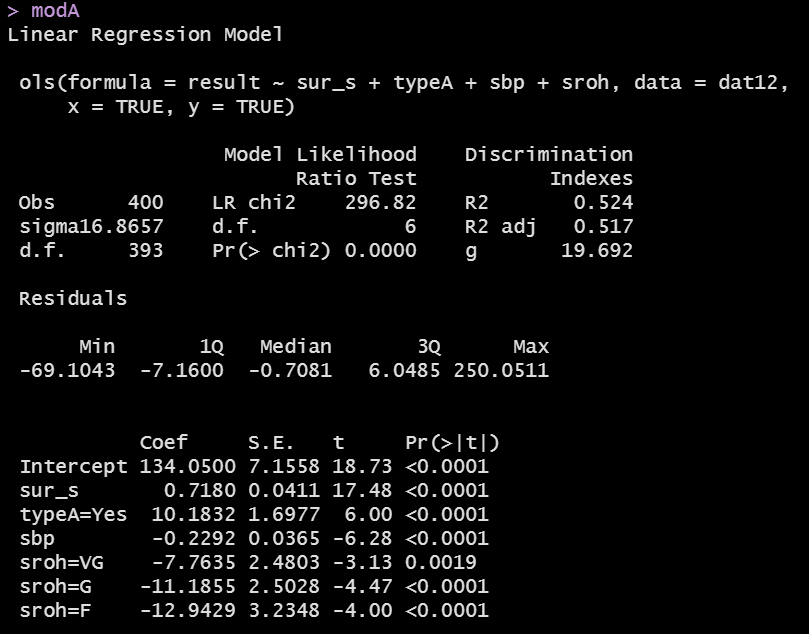
\includegraphics[width=11.24in,height=0.65\textheight]{figures/small1} \end{center}
\end{frame}

\begin{frame}[fragile]{ANOVA results for \texttt{modA}}
\protect\hypertarget{anova-results-for-moda}{}
\begin{Shaded}
\begin{Highlighting}[]
\FunctionTok{anova}\NormalTok{(modA)}
\end{Highlighting}
\end{Shaded}

\begin{verbatim}
                Analysis of Variance          Response: result 

 Factor     d.f. Partial SS MS         F      P     
 sur_s        1   86894.325 86894.3250 305.48 <.0001
 typeA        1   10233.702 10233.7022  35.98 <.0001
 sbp          1   11222.442 11222.4417  39.45 <.0001
 sroh         3    6825.387  2275.1291   8.00 <.0001
 REGRESSION   6  122994.902 20499.1504  72.07 <.0001
 ERROR      393  111789.458   284.4515              
\end{verbatim}
\end{frame}

\begin{frame}[fragile]{Plot Effect Sizes}
\protect\hypertarget{plot-effect-sizes}{}
\begin{Shaded}
\begin{Highlighting}[]
\FunctionTok{plot}\NormalTok{(}\FunctionTok{summary}\NormalTok{(modA))}
\end{Highlighting}
\end{Shaded}

\includegraphics{project_A_presentation_slides_files/figure-beamer/unnamed-chunk-9-1.pdf}
\end{frame}

\begin{frame}[fragile]{Consider Potential Non-Linear Terms}
\protect\hypertarget{consider-potential-non-linear-terms}{}
\begin{Shaded}
\begin{Highlighting}[]
\FunctionTok{plot}\NormalTok{(}\FunctionTok{spearman2}\NormalTok{(result }\SpecialCharTok{\textasciitilde{}}\NormalTok{ sur\_s }\SpecialCharTok{+}\NormalTok{ typeA }\SpecialCharTok{+}\NormalTok{ sbp }\SpecialCharTok{+}\NormalTok{ sroh, }
               \AttributeTok{data =}\NormalTok{ dat12))}
\end{Highlighting}
\end{Shaded}

\includegraphics{project_A_presentation_slides_files/figure-beamer/unnamed-chunk-10-1.pdf}
\end{frame}

\begin{frame}[fragile]{Using the Spearman plot as a guide\ldots{}}
\protect\hypertarget{using-the-spearman-plot-as-a-guide}{}
\begin{longtable}[]{@{}rll@{}}
\toprule
Variable & Description & Adj. Spearman \(\rho^2\) \\
\midrule
\endhead
\texttt{sur\_s} & Survey sur\_s (0-200 scale) & Highest \\
\texttt{typeA} & Type A (No or Yes) & 2nd Highest \\
\texttt{sbp} & Systolic Blood Pressure & 3rd Highest \\
\texttt{sroh} & Self-Reported Health (E/VG/G/F) & Lowest \\
\bottomrule
\end{longtable}

\begin{block}{Using Polynomials or Splines}
\protect\hypertarget{using-polynomials-or-splines}{}
\begin{itemize}
\tightlist
\item
  Can we build a (polynomial or spline) non-linear term that will add
  one more degree of freedom to our original main-effects model?
\item
  What if we can afford 2 additional df? Or 3?
\end{itemize}
\end{block}

\begin{block}{Using Interaction terms}
\protect\hypertarget{using-interaction-terms}{}
\begin{itemize}
\tightlist
\item
  How many df does the best categorical-categorical interaction use?
\item
  How many df does the best categorical-quantitative interaction use?
\end{itemize}
\end{block}
\end{frame}

\begin{frame}[fragile]{Adding Polynomial Terms in \texttt{sur\_s}}
\protect\hypertarget{adding-polynomial-terms-in-sur_s}{}
We'll look at a quadratic, then a cubic polynomial\ldots{}

\begin{Shaded}
\begin{Highlighting}[]
\NormalTok{modP2 }\OtherTok{\textless{}{-}} \FunctionTok{ols}\NormalTok{(result }\SpecialCharTok{\textasciitilde{}} \FunctionTok{pol}\NormalTok{(sur\_s,}\DecValTok{2}\NormalTok{) }\SpecialCharTok{+}\NormalTok{ typeA }\SpecialCharTok{+}\NormalTok{ sbp }\SpecialCharTok{+}\NormalTok{ sroh, }
               \AttributeTok{data =}\NormalTok{ dat12, }\AttributeTok{x =} \ConstantTok{TRUE}\NormalTok{, }\AttributeTok{y =} \ConstantTok{TRUE}\NormalTok{)}
\NormalTok{modP3 }\OtherTok{\textless{}{-}} \FunctionTok{ols}\NormalTok{(result }\SpecialCharTok{\textasciitilde{}} \FunctionTok{pol}\NormalTok{(sur\_s,}\DecValTok{3}\NormalTok{) }\SpecialCharTok{+}\NormalTok{ typeA }\SpecialCharTok{+}\NormalTok{ sbp }\SpecialCharTok{+}\NormalTok{ sroh, }
               \AttributeTok{data =}\NormalTok{ dat12, }\AttributeTok{x =} \ConstantTok{TRUE}\NormalTok{, }\AttributeTok{y =} \ConstantTok{TRUE}\NormalTok{)}
\end{Highlighting}
\end{Shaded}
\end{frame}

\begin{frame}[fragile]{Quadratic Polynomial adds 1 df to \texttt{modA}'s
6}
\protect\hypertarget{quadratic-polynomial-adds-1-df-to-modas-6}{}
\begin{Shaded}
\begin{Highlighting}[]
\NormalTok{modP2}
\end{Highlighting}
\end{Shaded}

\begin{center}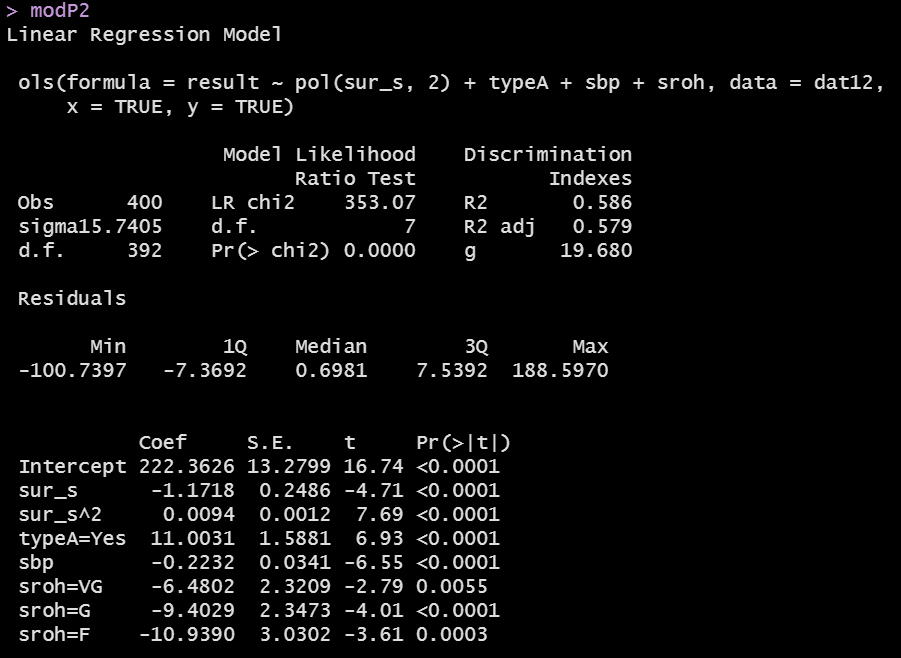
\includegraphics[width=12.51in,height=0.65\textheight]{figures/small2} \end{center}
\end{frame}

\begin{frame}[fragile]{Plot Effect Sizes}
\protect\hypertarget{plot-effect-sizes-1}{}
\begin{Shaded}
\begin{Highlighting}[]
\FunctionTok{plot}\NormalTok{(}\FunctionTok{summary}\NormalTok{(modP2))}
\end{Highlighting}
\end{Shaded}

\includegraphics{project_A_presentation_slides_files/figure-beamer/unnamed-chunk-14-1.pdf}
\end{frame}

\begin{frame}[fragile]{What does model \texttt{modA} look like?}
\protect\hypertarget{what-does-model-moda-look-like}{}
\begin{Shaded}
\begin{Highlighting}[]
\FunctionTok{ggplot}\NormalTok{(}\FunctionTok{Predict}\NormalTok{(modA))}
\end{Highlighting}
\end{Shaded}

\includegraphics{project_A_presentation_slides_files/figure-beamer/unnamed-chunk-15-1.pdf}
\end{frame}

\begin{frame}[fragile]{What does model \texttt{modP2} look like?}
\protect\hypertarget{what-does-model-modp2-look-like}{}
\begin{Shaded}
\begin{Highlighting}[]
\FunctionTok{ggplot}\NormalTok{(}\FunctionTok{Predict}\NormalTok{(modP2))}
\end{Highlighting}
\end{Shaded}

\includegraphics{project_A_presentation_slides_files/figure-beamer/unnamed-chunk-16-1.pdf}
\end{frame}

\begin{frame}[fragile]{Nomogram for model \texttt{modA}}
\protect\hypertarget{nomogram-for-model-moda}{}
\begin{Shaded}
\begin{Highlighting}[]
\FunctionTok{plot}\NormalTok{(}\FunctionTok{nomogram}\NormalTok{(modA))}
\end{Highlighting}
\end{Shaded}

\includegraphics{project_A_presentation_slides_files/figure-beamer/unnamed-chunk-17-1.pdf}
\end{frame}

\begin{frame}[fragile]{Nomogram for model \texttt{modP2}}
\protect\hypertarget{nomogram-for-model-modp2}{}
\begin{Shaded}
\begin{Highlighting}[]
\FunctionTok{plot}\NormalTok{(}\FunctionTok{nomogram}\NormalTok{(modP2))}
\end{Highlighting}
\end{Shaded}

\includegraphics{project_A_presentation_slides_files/figure-beamer/unnamed-chunk-18-1.pdf}
\end{frame}

\begin{frame}[fragile]{Do the non-linear terms in \texttt{modP2} do
much?}
\protect\hypertarget{do-the-non-linear-terms-in-modp2-do-much}{}
\begin{Shaded}
\begin{Highlighting}[]
\FunctionTok{anova}\NormalTok{(modP2)}
\end{Highlighting}
\end{Shaded}

\begin{verbatim}
                Analysis of Variance          Response: result 

 Factor     d.f. Partial SS MS         F      P     
 sur_s        2  101560.602 50780.3008 204.95 <.0001
  Nonlinear   1   14666.277 14666.2767  59.19 <.0001
 typeA        1   11894.005 11894.0047  48.01 <.0001
 sbp          1   10636.075 10636.0753  42.93 <.0001
 sroh         3    4795.273  1598.4244   6.45 3e-04 
 REGRESSION   7  137661.179 19665.8827  79.37 <.0001
 ERROR      392   97123.181   247.7632              
\end{verbatim}
\end{frame}

\begin{frame}[fragile]{Do the non-linear terms in \texttt{modP2} help
much?}
\protect\hypertarget{do-the-non-linear-terms-in-modp2-help-much}{}
\begin{Shaded}
\begin{Highlighting}[]
\FunctionTok{AIC}\NormalTok{(modA); }\FunctionTok{BIC}\NormalTok{(modA)}
\end{Highlighting}
\end{Shaded}

\begin{verbatim}
    d.f. 
3404.314 
\end{verbatim}

\begin{verbatim}
    d.f. 
3436.246 
\end{verbatim}

\begin{Shaded}
\begin{Highlighting}[]
\FunctionTok{AIC}\NormalTok{(modP2); }\FunctionTok{BIC}\NormalTok{(modP2)}
\end{Highlighting}
\end{Shaded}

\begin{verbatim}
    d.f. 
3350.059 
\end{verbatim}

\begin{verbatim}
    d.f. 
3385.982 
\end{verbatim}
\end{frame}

\begin{frame}[fragile]{Cubic (degree 3) polynomial adds 2 df to
\texttt{modA}'s 6}
\protect\hypertarget{cubic-degree-3-polynomial-adds-2-df-to-modas-6}{}
\begin{Shaded}
\begin{Highlighting}[]
\NormalTok{modP3}
\end{Highlighting}
\end{Shaded}

\begin{center}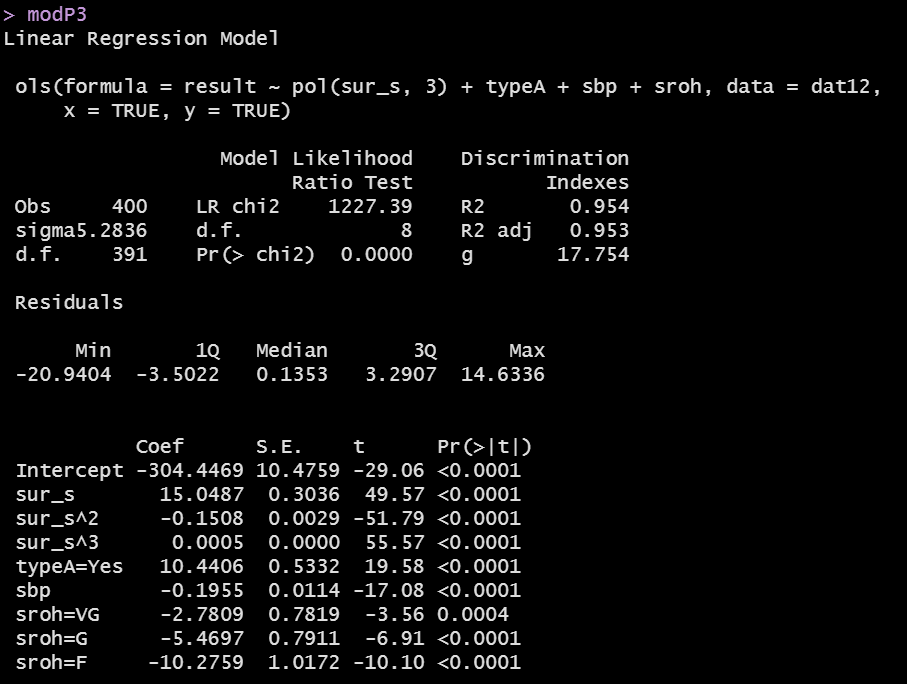
\includegraphics[width=12.6in,height=0.65\textheight]{figures/small3} \end{center}
\end{frame}

\begin{frame}[fragile]{What does model \texttt{modP3} look like?}
\protect\hypertarget{what-does-model-modp3-look-like}{}
\begin{Shaded}
\begin{Highlighting}[]
\FunctionTok{ggplot}\NormalTok{(}\FunctionTok{Predict}\NormalTok{(modP3))}
\end{Highlighting}
\end{Shaded}

\includegraphics{project_A_presentation_slides_files/figure-beamer/unnamed-chunk-23-1.pdf}
\end{frame}

\begin{frame}[fragile]{Nomogram for model \texttt{modP3}}
\protect\hypertarget{nomogram-for-model-modp3}{}
\begin{Shaded}
\begin{Highlighting}[]
\FunctionTok{plot}\NormalTok{(}\FunctionTok{nomogram}\NormalTok{(modP3))}
\end{Highlighting}
\end{Shaded}

\includegraphics{project_A_presentation_slides_files/figure-beamer/unnamed-chunk-24-1.pdf}
\end{frame}

\begin{frame}[fragile]{How about a restricted cubic spline in
\texttt{cigs}?}
\protect\hypertarget{how-about-a-restricted-cubic-spline-in-cigs}{}
\begin{Shaded}
\begin{Highlighting}[]
\NormalTok{modC3 }\OtherTok{\textless{}{-}} \FunctionTok{ols}\NormalTok{(result }\SpecialCharTok{\textasciitilde{}} \FunctionTok{rcs}\NormalTok{(sur\_s,}\DecValTok{3}\NormalTok{) }\SpecialCharTok{+}\NormalTok{ typeA }\SpecialCharTok{+}\NormalTok{ sbp }\SpecialCharTok{+}\NormalTok{ sroh, }
               \AttributeTok{data =}\NormalTok{ dat12, }\AttributeTok{x =} \ConstantTok{TRUE}\NormalTok{, }\AttributeTok{y =} \ConstantTok{TRUE}\NormalTok{)}
\NormalTok{modC4 }\OtherTok{\textless{}{-}} \FunctionTok{ols}\NormalTok{(result }\SpecialCharTok{\textasciitilde{}} \FunctionTok{rcs}\NormalTok{(sur\_s,}\DecValTok{4}\NormalTok{) }\SpecialCharTok{+}\NormalTok{ typeA }\SpecialCharTok{+}\NormalTok{ sbp }\SpecialCharTok{+}\NormalTok{ sroh, }
               \AttributeTok{data =}\NormalTok{ dat12, }\AttributeTok{x =} \ConstantTok{TRUE}\NormalTok{, }\AttributeTok{y =} \ConstantTok{TRUE}\NormalTok{)}
\NormalTok{modC5 }\OtherTok{\textless{}{-}} \FunctionTok{ols}\NormalTok{(result }\SpecialCharTok{\textasciitilde{}} \FunctionTok{rcs}\NormalTok{(sur\_s,}\DecValTok{5}\NormalTok{) }\SpecialCharTok{+}\NormalTok{ typeA }\SpecialCharTok{+}\NormalTok{ sbp }\SpecialCharTok{+}\NormalTok{ sroh, }
               \AttributeTok{data =}\NormalTok{ dat12, }\AttributeTok{x =} \ConstantTok{TRUE}\NormalTok{, }\AttributeTok{y =} \ConstantTok{TRUE}\NormalTok{)}
\end{Highlighting}
\end{Shaded}
\end{frame}

\begin{frame}[fragile]{RCS with 3 knots adds 1 df to \texttt{modA}'s 6}
\protect\hypertarget{rcs-with-3-knots-adds-1-df-to-modas-6}{}
\begin{Shaded}
\begin{Highlighting}[]
\NormalTok{modC3}
\end{Highlighting}
\end{Shaded}

\begin{center}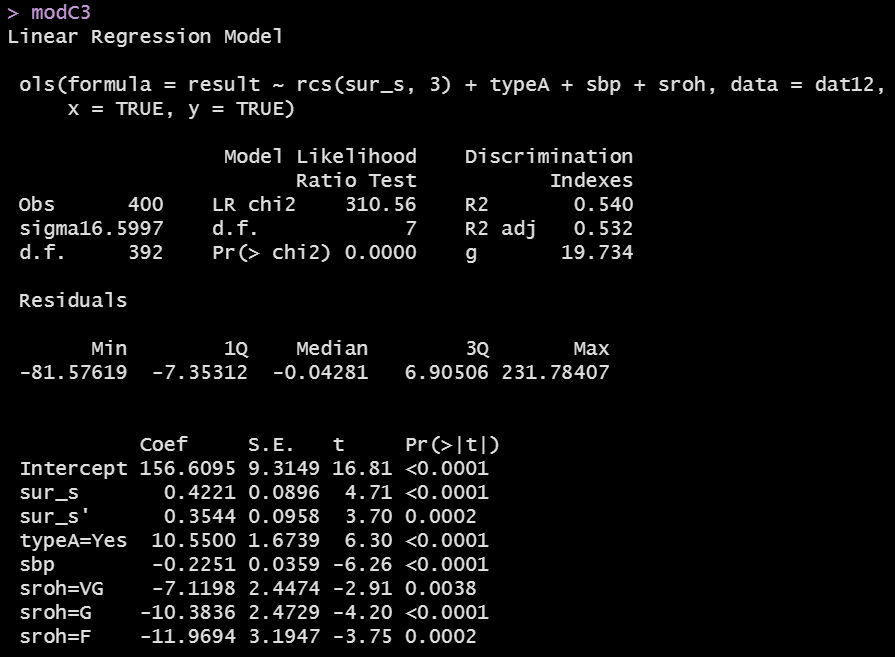
\includegraphics[width=12.43in,height=0.65\textheight]{figures/small4} \end{center}
\end{frame}

\begin{frame}[fragile]{What does model \texttt{modC3} look like?}
\protect\hypertarget{what-does-model-modc3-look-like}{}
\begin{Shaded}
\begin{Highlighting}[]
\FunctionTok{ggplot}\NormalTok{(}\FunctionTok{Predict}\NormalTok{(modC3))}
\end{Highlighting}
\end{Shaded}

\includegraphics{project_A_presentation_slides_files/figure-beamer/unnamed-chunk-28-1.pdf}
\end{frame}

\begin{frame}[fragile]{What does the nomogram for \texttt{modC3} look
like?}
\protect\hypertarget{what-does-the-nomogram-for-modc3-look-like}{}
\begin{Shaded}
\begin{Highlighting}[]
\FunctionTok{plot}\NormalTok{(}\FunctionTok{nomogram}\NormalTok{(modC3))}
\end{Highlighting}
\end{Shaded}

\includegraphics{project_A_presentation_slides_files/figure-beamer/unnamed-chunk-29-1.pdf}
\end{frame}

\begin{frame}[fragile]{Do the non-linear terms help much in
\texttt{modC3}?}
\protect\hypertarget{do-the-non-linear-terms-help-much-in-modc3}{}
\begin{Shaded}
\begin{Highlighting}[]
\FunctionTok{AIC}\NormalTok{(modC3); }\FunctionTok{BIC}\NormalTok{(modC3)}
\end{Highlighting}
\end{Shaded}

\begin{verbatim}
    d.f. 
3392.579 
\end{verbatim}

\begin{verbatim}
    d.f. 
3428.502 
\end{verbatim}

\begin{Shaded}
\begin{Highlighting}[]
\FunctionTok{AIC}\NormalTok{(modA); }\FunctionTok{BIC}\NormalTok{(modA)}
\end{Highlighting}
\end{Shaded}

\begin{verbatim}
    d.f. 
3404.314 
\end{verbatim}

\begin{verbatim}
    d.f. 
3436.246 
\end{verbatim}
\end{frame}

\begin{frame}[fragile]{ANOVA table for \texttt{modC3}?}
\protect\hypertarget{anova-table-for-modc3}{}
\begin{Shaded}
\begin{Highlighting}[]
\FunctionTok{anova}\NormalTok{(modC3)}
\end{Highlighting}
\end{Shaded}

\begin{verbatim}
                Analysis of Variance          Response: result 

 Factor     d.f. Partial SS MS         F      P     
 sur_s        2   90667.755 45333.8775 164.52 <.0001
  Nonlinear   1    3773.430  3773.4300  13.69 2e-04 
 typeA        1   10945.709 10945.7087  39.72 <.0001
 sbp          1   10806.525 10806.5247  39.22 <.0001
 sroh         3    5820.777  1940.2589   7.04 1e-04 
 REGRESSION   7  126768.332 18109.7617  65.72 <.0001
 ERROR      392  108016.028   275.5511              
\end{verbatim}
\end{frame}

\begin{frame}[fragile]{RCS with 4 knots adds 2 df to \texttt{modA}'s 6}
\protect\hypertarget{rcs-with-4-knots-adds-2-df-to-modas-6}{}
\begin{Shaded}
\begin{Highlighting}[]
\NormalTok{modC4}
\end{Highlighting}
\end{Shaded}

\begin{center}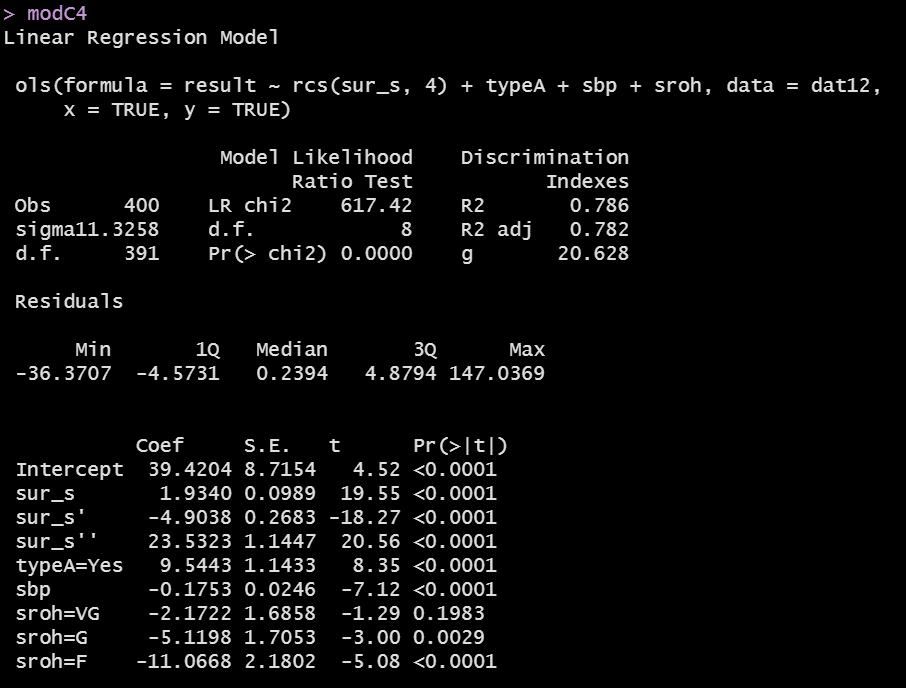
\includegraphics[width=12.58in,height=0.65\textheight]{figures/small5} \end{center}
\end{frame}

\begin{frame}[fragile]{What does model \texttt{modC4} look like?}
\protect\hypertarget{what-does-model-modc4-look-like}{}
\begin{Shaded}
\begin{Highlighting}[]
\FunctionTok{ggplot}\NormalTok{(}\FunctionTok{Predict}\NormalTok{(modC4))}
\end{Highlighting}
\end{Shaded}

\includegraphics{project_A_presentation_slides_files/figure-beamer/unnamed-chunk-34-1.pdf}
\end{frame}

\begin{frame}[fragile]{What does the nomogram for \texttt{modC4} look
like?}
\protect\hypertarget{what-does-the-nomogram-for-modc4-look-like}{}
\begin{Shaded}
\begin{Highlighting}[]
\FunctionTok{plot}\NormalTok{(}\FunctionTok{nomogram}\NormalTok{(modC4))}
\end{Highlighting}
\end{Shaded}

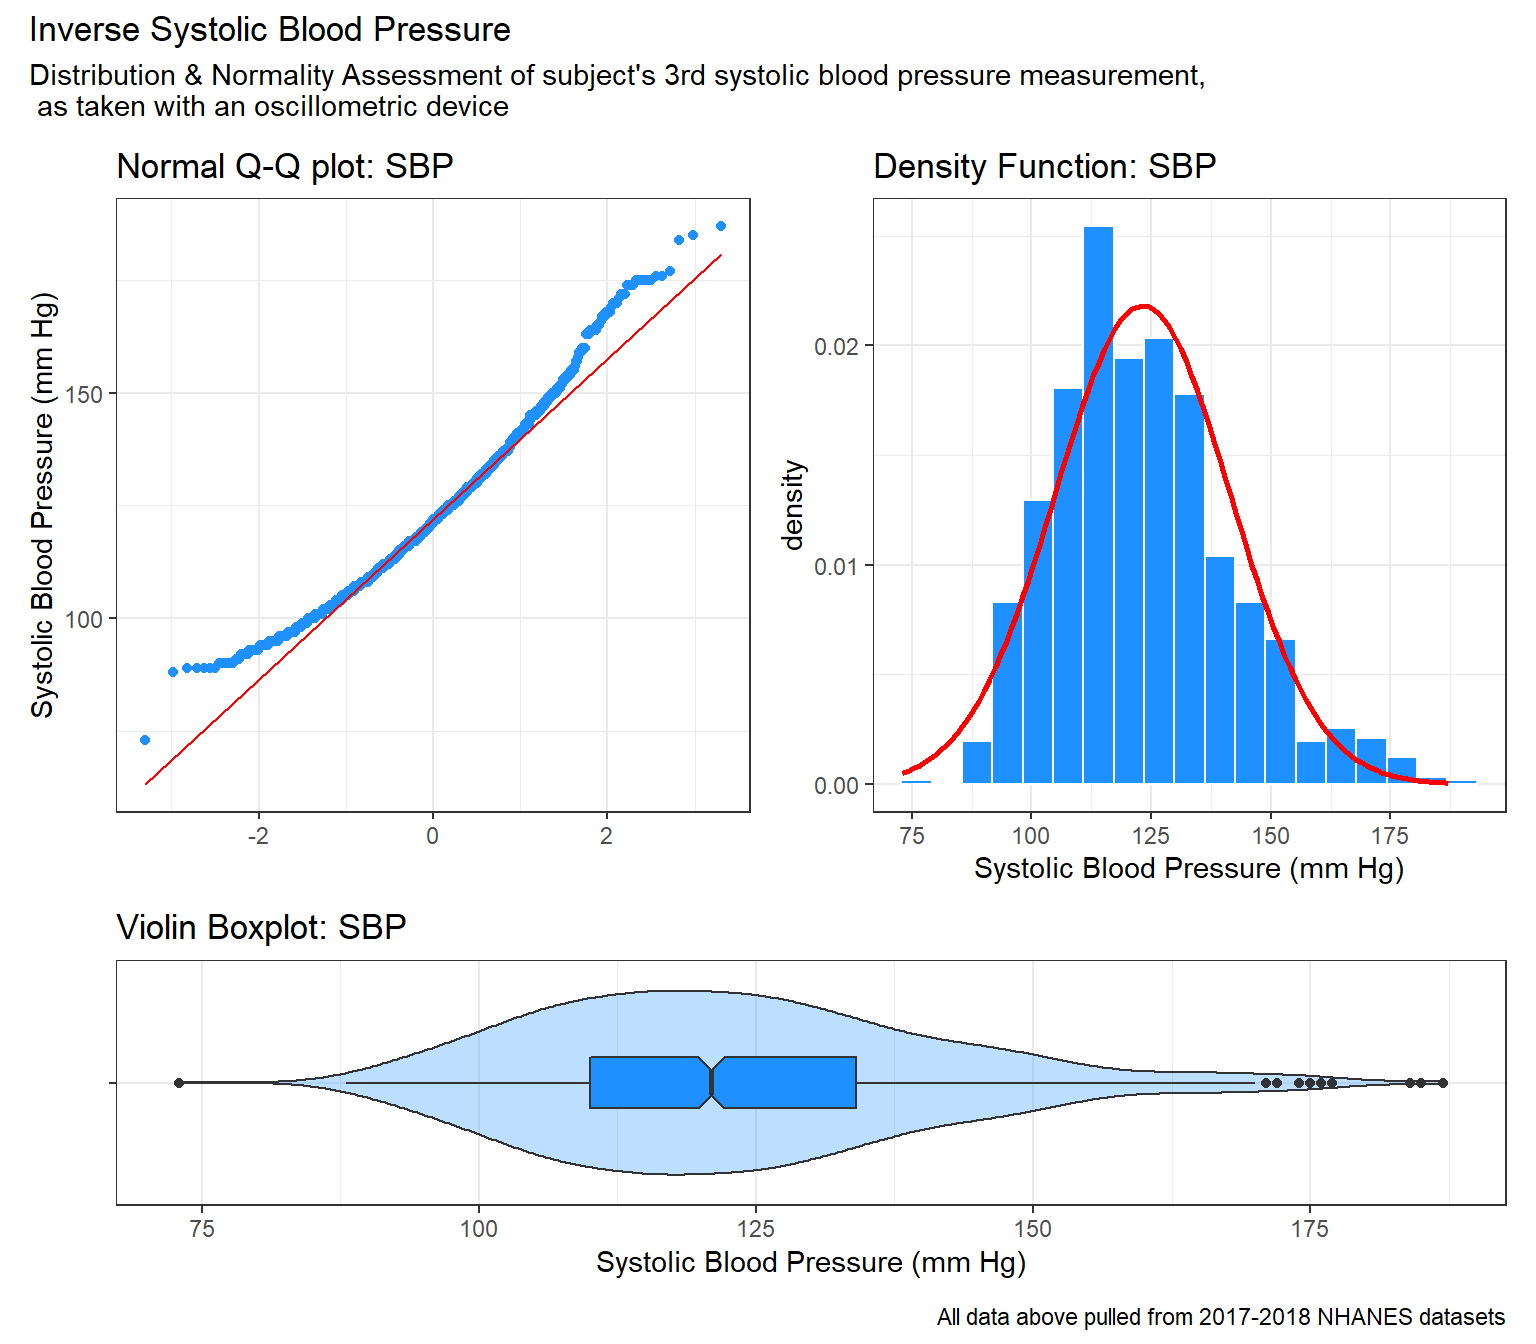
\includegraphics{project_A_presentation_slides_files/figure-beamer/unnamed-chunk-35-1.pdf}
\end{frame}

\begin{frame}[fragile]{RCS with 5 knots adds 3 df to \texttt{modA}'s 6}
\protect\hypertarget{rcs-with-5-knots-adds-3-df-to-modas-6}{}
\begin{Shaded}
\begin{Highlighting}[]
\NormalTok{modC5}
\end{Highlighting}
\end{Shaded}

\begin{center}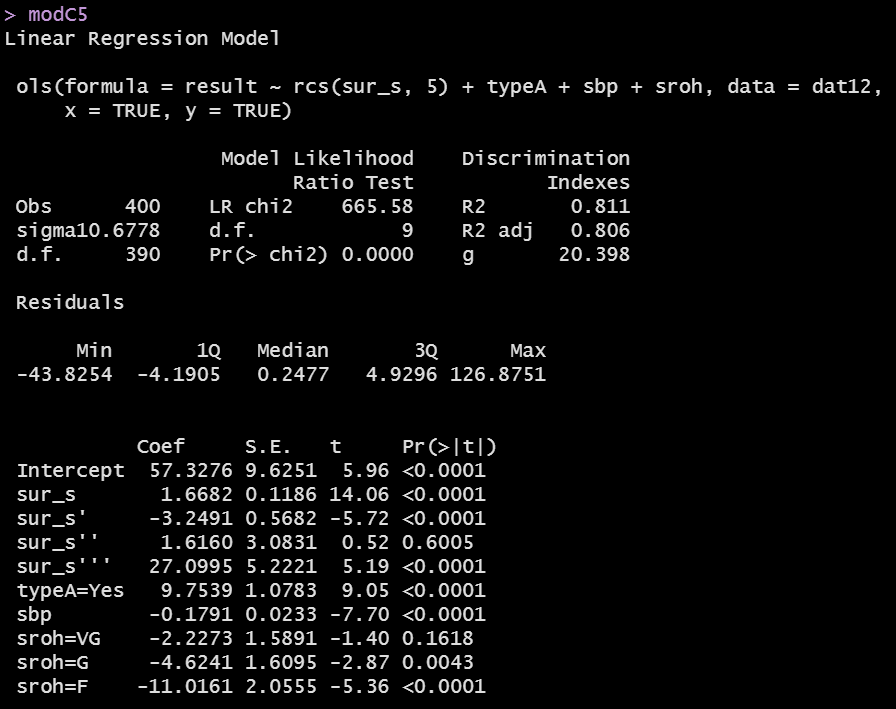
\includegraphics[width=12.44in,height=0.65\textheight]{figures/small6} \end{center}
\end{frame}

\begin{frame}[fragile]{What does model \texttt{modC5} look like?}
\protect\hypertarget{what-does-model-modc5-look-like}{}
\begin{Shaded}
\begin{Highlighting}[]
\FunctionTok{ggplot}\NormalTok{(}\FunctionTok{Predict}\NormalTok{(modC5))}
\end{Highlighting}
\end{Shaded}

\includegraphics{project_A_presentation_slides_files/figure-beamer/unnamed-chunk-38-1.pdf}
\end{frame}

\begin{frame}[fragile]{What does the nomogram for \texttt{modC5} look
like?}
\protect\hypertarget{what-does-the-nomogram-for-modc5-look-like}{}
\begin{Shaded}
\begin{Highlighting}[]
\FunctionTok{plot}\NormalTok{(}\FunctionTok{nomogram}\NormalTok{(modC5))}
\end{Highlighting}
\end{Shaded}

\includegraphics{project_A_presentation_slides_files/figure-beamer/unnamed-chunk-39-1.pdf}
\end{frame}

\begin{frame}[fragile]{Splines and Polynomials with \texttt{ols} (or
\texttt{lrm})}
\protect\hypertarget{splines-and-polynomials-with-ols-or-lrm}{}
\begin{longtable}[]{@{}rccc@{}}
\toprule
Model & Coeffs. & ``Bends'' & DF added \\
\midrule
\endhead
Main Effects (\texttt{modA}) & None & None & -- \\
Polynomial, degree 2 (\texttt{P2}) & \texttt{\^{}2} & 1 & 1 \\
Polynomial, degree 3 (\texttt{P3}) & \texttt{\^{}2,\ \^{}3} & 2 & 2 \\
RCS, 3 knots (\texttt{C3}) & \texttt{\textquotesingle{}} & 2 & 1 \\
RCS, 4 knots (\texttt{C4}) &
\texttt{\textquotesingle{},\ \textquotesingle{}\textquotesingle{}} & 3 &
2 \\
RCS, 5 knots (\texttt{C5}) &
\texttt{\textquotesingle{},\ \textquotesingle{}\textquotesingle{},\ \textquotesingle{}\textquotesingle{}\textquotesingle{}}
& 4 & 3 \\
\bottomrule
\end{longtable}

\begin{itemize}
\tightlist
\item
  RCS = Restricted Cubic Spline
\end{itemize}
\end{frame}

\begin{frame}[fragile]{What about an interaction term instead?}
\protect\hypertarget{what-about-an-interaction-term-instead}{}
\begin{enumerate}
\tightlist
\item
  How many df does the best categorical-categorical interaction use?
\item
  How many df does the best categorical-quantitative interaction use?
\end{enumerate}

\begin{Shaded}
\begin{Highlighting}[]
\FunctionTok{plot}\NormalTok{(}\FunctionTok{spearman2}\NormalTok{(result }\SpecialCharTok{\textasciitilde{}}\NormalTok{ sur\_s }\SpecialCharTok{+}\NormalTok{ typeA }\SpecialCharTok{+}\NormalTok{ sbp }\SpecialCharTok{+}\NormalTok{ sroh, }
               \AttributeTok{data =}\NormalTok{ dat12))}
\end{Highlighting}
\end{Shaded}

\includegraphics{project_A_presentation_slides_files/figure-beamer/unnamed-chunk-40-1.pdf}
\end{frame}

\begin{frame}[fragile]{Models with Interaction Terms}
\protect\hypertarget{models-with-interaction-terms}{}
\begin{Shaded}
\begin{Highlighting}[]
\CommentTok{\# already set up datadist for dat12}

\NormalTok{modI1 }\OtherTok{\textless{}{-}} \FunctionTok{ols}\NormalTok{(result }\SpecialCharTok{\textasciitilde{}}\NormalTok{ sur\_s }\SpecialCharTok{*}\NormalTok{ typeA }\SpecialCharTok{+}\NormalTok{ sbp }\SpecialCharTok{+}\NormalTok{ sroh,}
             \AttributeTok{data =}\NormalTok{ dat12, }\AttributeTok{x =} \ConstantTok{TRUE}\NormalTok{, }\AttributeTok{y =} \ConstantTok{TRUE}\NormalTok{)}
\NormalTok{modI2 }\OtherTok{\textless{}{-}} \FunctionTok{ols}\NormalTok{(result }\SpecialCharTok{\textasciitilde{}} \FunctionTok{rcs}\NormalTok{(sur\_s, }\DecValTok{4}\NormalTok{) }\SpecialCharTok{+}\NormalTok{ typeA }\SpecialCharTok{+} 
\NormalTok{                 sur\_s }\SpecialCharTok{\%ia\%}\NormalTok{ typeA }\SpecialCharTok{+}\NormalTok{ sbp }\SpecialCharTok{+}\NormalTok{ sroh, }
             \AttributeTok{data =}\NormalTok{ dat12, }\AttributeTok{x =} \ConstantTok{TRUE}\NormalTok{, }\AttributeTok{y =} \ConstantTok{TRUE}\NormalTok{)}
\end{Highlighting}
\end{Shaded}
\end{frame}

\begin{frame}[fragile]{Model \texttt{modI1} adds how many df to
\texttt{modA}?}
\protect\hypertarget{model-modi1-adds-how-many-df-to-moda}{}
\begin{Shaded}
\begin{Highlighting}[]
\NormalTok{modI1}
\end{Highlighting}
\end{Shaded}

\begin{center}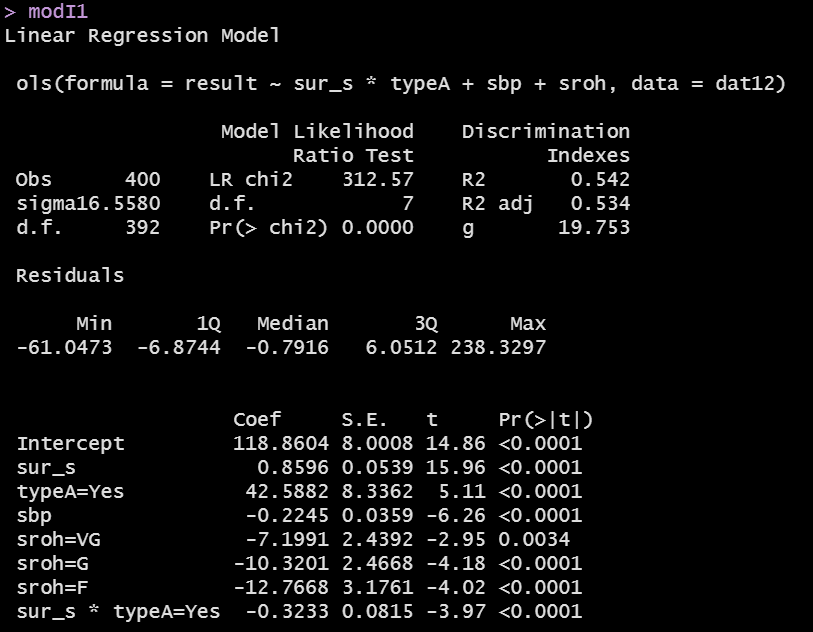
\includegraphics[width=11.29in,height=0.65\textheight]{figures/small7} \end{center}
\end{frame}

\begin{frame}[fragile]{ANOVA for \texttt{modI1}}
\protect\hypertarget{anova-for-modi1}{}
\begin{Shaded}
\begin{Highlighting}[]
\FunctionTok{anova}\NormalTok{(modI1)}
\end{Highlighting}
\end{Shaded}

\begin{center}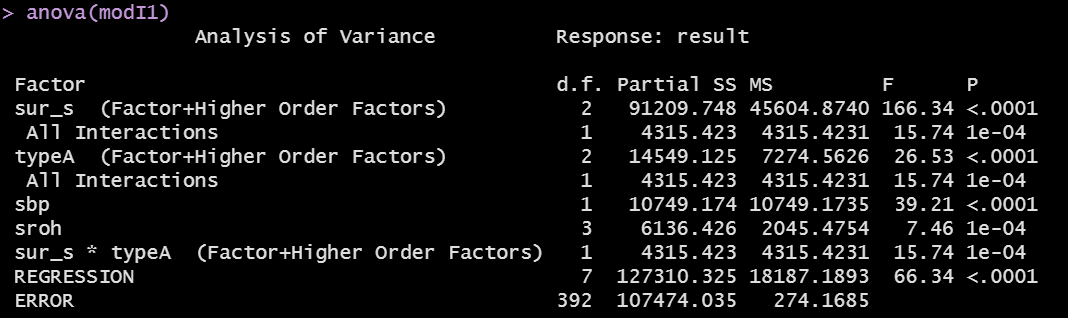
\includegraphics[width=0.85\linewidth]{figures/small7b} \end{center}
\end{frame}

\begin{frame}[fragile]{What does \texttt{modI1} look like?}
\protect\hypertarget{what-does-modi1-look-like}{}
\begin{Shaded}
\begin{Highlighting}[]
\FunctionTok{ggplot}\NormalTok{(}\FunctionTok{Predict}\NormalTok{(modI1))}
\end{Highlighting}
\end{Shaded}

\includegraphics{project_A_presentation_slides_files/figure-beamer/unnamed-chunk-46-1.pdf}
\end{frame}

\begin{frame}[fragile]{Nomogram for \texttt{modI1}}
\protect\hypertarget{nomogram-for-modi1}{}
\begin{Shaded}
\begin{Highlighting}[]
\FunctionTok{plot}\NormalTok{(}\FunctionTok{nomogram}\NormalTok{(modI1))}
\end{Highlighting}
\end{Shaded}

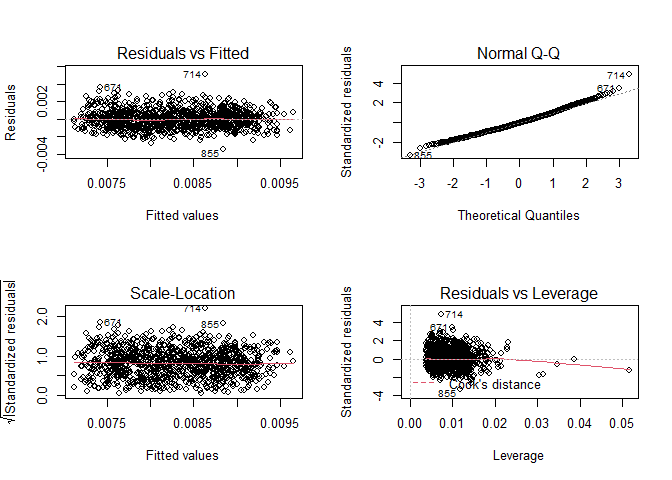
\includegraphics{project_A_presentation_slides_files/figure-beamer/unnamed-chunk-47-1.pdf}
\end{frame}

\begin{frame}[fragile]{Model \texttt{modI2} adds how many df to
\texttt{modC4}?}
\protect\hypertarget{model-modi2-adds-how-many-df-to-modc4}{}
\begin{Shaded}
\begin{Highlighting}[]
\NormalTok{modI2}
\end{Highlighting}
\end{Shaded}

\begin{center}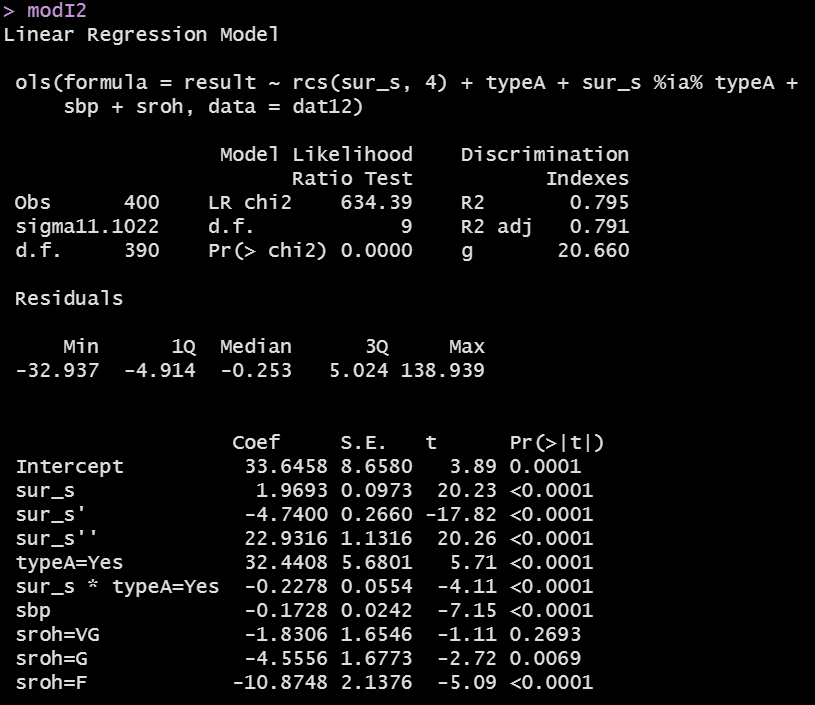
\includegraphics[width=11.32in,height=0.65\textheight]{figures/small8} \end{center}
\end{frame}

\begin{frame}[fragile]{ANOVA for \texttt{modI2}}
\protect\hypertarget{anova-for-modi2}{}
\begin{Shaded}
\begin{Highlighting}[]
\FunctionTok{anova}\NormalTok{(modI2)}
\end{Highlighting}
\end{Shaded}

\begin{center}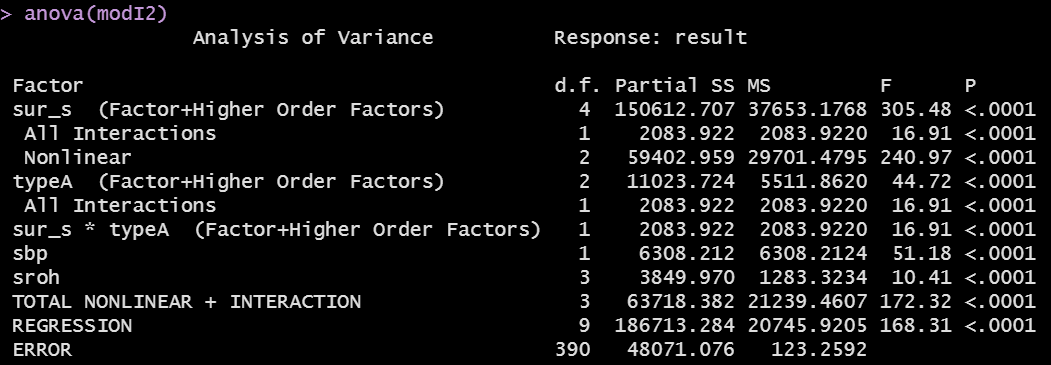
\includegraphics[width=0.85\linewidth]{figures/small8b} \end{center}
\end{frame}

\begin{frame}[fragile]{What does \texttt{modI2} look like?}
\protect\hypertarget{what-does-modi2-look-like}{}
\begin{Shaded}
\begin{Highlighting}[]
\FunctionTok{ggplot}\NormalTok{(}\FunctionTok{Predict}\NormalTok{(modI2))}
\end{Highlighting}
\end{Shaded}

\includegraphics{project_A_presentation_slides_files/figure-beamer/unnamed-chunk-52-1.pdf}
\end{frame}

\begin{frame}[fragile]{Nomogram for \texttt{modI2}}
\protect\hypertarget{nomogram-for-modi2}{}
\begin{Shaded}
\begin{Highlighting}[]
\FunctionTok{plot}\NormalTok{(}\FunctionTok{nomogram}\NormalTok{(modI2))}
\end{Highlighting}
\end{Shaded}

\includegraphics{project_A_presentation_slides_files/figure-beamer/unnamed-chunk-53-1.pdf}
\end{frame}

\begin{frame}[fragile]{Comparing Models?}
\protect\hypertarget{comparing-models}{}
\begin{Shaded}
\begin{Highlighting}[]
\FunctionTok{set.seed}\NormalTok{(}\DecValTok{4321}\NormalTok{); }\FunctionTok{validate}\NormalTok{(modA)}
\end{Highlighting}
\end{Shaded}

\begin{verbatim}
          index.orig training     test optimism
R-square      0.5239   0.5485   0.5035   0.0450
MSE         279.4736 309.0788 291.4385  17.6403
g            19.6922  20.4852  19.5334   0.9518
Intercept     0.0000   0.0000   5.5331  -5.5331
Slope         1.0000   1.0000   0.9670   0.0330
          index.corrected  n
R-square           0.4788 40
MSE              261.8333 40
g                 18.7404 40
Intercept          5.5331 40
Slope              0.9670 40
\end{verbatim}

\begin{itemize}
\tightlist
\item
  Ran validate for other models (see next slide)
\end{itemize}
\end{frame}

\begin{frame}[fragile]{Table of \texttt{validate} Results}
\protect\hypertarget{table-of-validate-results}{}
\begin{longtable}[]{@{}lrrr@{}}
\toprule
Model & Raw \(R^2\) & Corrected \(R^2\) & Corrected MSE \\
\midrule
\endhead
\texttt{modA} (Main Effects) & 0.5239 & 0.4788 & 261.8 \\
\texttt{modP2} (Quadr. Pol.) & 0.5863 & 0.4756 & 293.8 \\
\texttt{modP3} (Cubic Pol.) & 0.9535 & 0.9684 & 28.5 \\
\texttt{modC3} (RCS, 3 knots) & 0.5399 & 0.4510 & 313.0 \\
\texttt{modC4} (RCS, 4 knots) & 0.7864 & 0.7294 & 162.8 \\
\texttt{modC5} (RCS, 5 knots) & 0.8106 & 0.7580 & 137.6 \\
\texttt{modI1} (interaction) & 0.5422 & 0.4413 & 339.2 \\
\texttt{modI2} (int + RCS4) & 0.7953 & 0.7337 & 161.4 \\
\bottomrule
\end{longtable}
\end{frame}

\begin{frame}[fragile]{Making Predictions}
\protect\hypertarget{making-predictions}{}
Suppose we want to predict the \texttt{result} for these new subjects:

\begin{Shaded}
\begin{Highlighting}[]
\NormalTok{new\_people }\OtherTok{\textless{}{-}} \FunctionTok{tibble}\NormalTok{(}
    \AttributeTok{name =} \FunctionTok{c}\NormalTok{(}\StringTok{"Dave"}\NormalTok{, }\StringTok{"Edna"}\NormalTok{),}
    \AttributeTok{sur\_s =} \FunctionTok{c}\NormalTok{(}\DecValTok{100}\NormalTok{, }\DecValTok{115}\NormalTok{), }\AttributeTok{typeA =} \FunctionTok{c}\NormalTok{(}\StringTok{"Yes"}\NormalTok{, }\StringTok{"No"}\NormalTok{),}
    \AttributeTok{sbp =} \FunctionTok{c}\NormalTok{(}\DecValTok{140}\NormalTok{, }\DecValTok{125}\NormalTok{), }\AttributeTok{sroh =} \FunctionTok{c}\NormalTok{(}\StringTok{"G"}\NormalTok{, }\StringTok{"E"}\NormalTok{))}

\NormalTok{new\_people }\SpecialCharTok{\%\textgreater{}\%} \FunctionTok{kable}\NormalTok{()}
\end{Highlighting}
\end{Shaded}

\begin{longtable}[]{@{}lrlrl@{}}
\toprule
name & sur\_s & typeA & sbp & sroh \\
\midrule
\endhead
Dave & 100 & Yes & 140 & G \\
Edna & 115 & No & 125 & E \\
\bottomrule
\end{longtable}
\end{frame}

\begin{frame}[fragile]{Predicting Dave and Edna with \texttt{modA}}
\protect\hypertarget{predicting-dave-and-edna-with-moda}{}
\begin{itemize}
\tightlist
\item
  Individual Prediction Intervals
\end{itemize}

\begin{Shaded}
\begin{Highlighting}[]
\FunctionTok{predict}\NormalTok{(modA, }\AttributeTok{newdata =} \FunctionTok{data.frame}\NormalTok{(new\_people), }
        \AttributeTok{conf.int =} \FloatTok{0.95}\NormalTok{, }\AttributeTok{conf.type =} \StringTok{"individual"}\NormalTok{)}
\end{Highlighting}
\end{Shaded}

\begin{verbatim}
$linear.predictors
       1        2 
172.7522 187.9628 

$lower
       1        2 
139.4297 154.4792 

$upper
       1        2 
206.0747 221.4463 
\end{verbatim}
\end{frame}

\begin{frame}[fragile]{Predicting mean of people just like Dave and Edna
with \texttt{modA}}
\protect\hypertarget{predicting-mean-of-people-just-like-dave-and-edna-with-moda}{}
\begin{itemize}
\tightlist
\item
  Mean Prediction Intervals
\end{itemize}

\begin{Shaded}
\begin{Highlighting}[]
\FunctionTok{predict}\NormalTok{(modA, }\AttributeTok{newdata =} \FunctionTok{data.frame}\NormalTok{(new\_people), }
        \AttributeTok{conf.int =} \FloatTok{0.95}\NormalTok{, }\AttributeTok{conf.type =} \StringTok{"mean"}\NormalTok{)}
\end{Highlighting}
\end{Shaded}

\begin{verbatim}
$linear.predictors
       1        2 
172.7522 187.9628 

$lower
       1        2 
169.4477 183.3068 

$upper
       1        2 
176.0567 192.6188 
\end{verbatim}
\end{frame}

\begin{frame}[fragile]{Predicting Dave and Edna with other models}
\protect\hypertarget{predicting-dave-and-edna-with-other-models}{}
\begin{Shaded}
\begin{Highlighting}[]
\FunctionTok{predict}\NormalTok{(modP3, }\AttributeTok{newdata =} \FunctionTok{data.frame}\NormalTok{(new\_people))}
\end{Highlighting}
\end{Shaded}

\begin{verbatim}
       1        2 
173.8945 173.7410 
\end{verbatim}

\begin{Shaded}
\begin{Highlighting}[]
\FunctionTok{predict}\NormalTok{(modC4, }\AttributeTok{newdata =} \FunctionTok{data.frame}\NormalTok{(new\_people))}
\end{Highlighting}
\end{Shaded}

\begin{verbatim}
       1        2 
171.7091 167.9763 
\end{verbatim}

\begin{Shaded}
\begin{Highlighting}[]
\FunctionTok{predict}\NormalTok{(modI2, }\AttributeTok{newdata =} \FunctionTok{data.frame}\NormalTok{(new\_people))}
\end{Highlighting}
\end{Shaded}

\begin{verbatim}
       1        2 
171.8875 169.4290 
\end{verbatim}
\end{frame}

\begin{frame}[fragile]{Predicting Dave via the Nomogram for model
\texttt{modC3}}
\protect\hypertarget{predicting-dave-via-the-nomogram-for-model-modc3}{}
\begin{itemize}
\tightlist
\item
  Dave has \texttt{sur\_s} = 100, is typeA, Good \texttt{sroh},
  \texttt{sbp} = 140.
\end{itemize}

\begin{Shaded}
\begin{Highlighting}[]
\FunctionTok{plot}\NormalTok{(}\FunctionTok{nomogram}\NormalTok{(modC3))}
\end{Highlighting}
\end{Shaded}

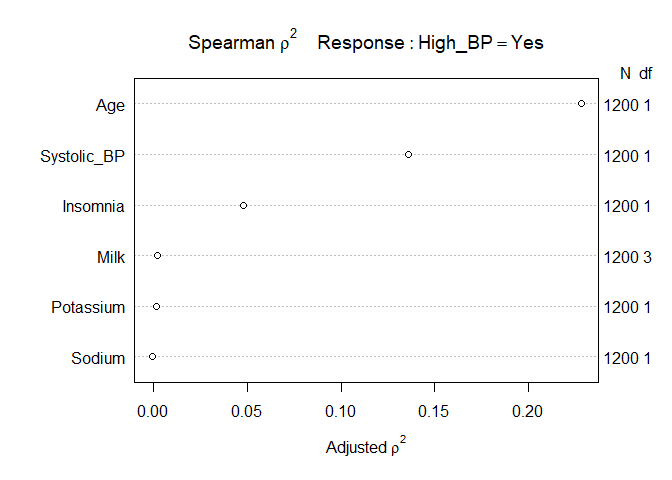
\includegraphics{project_A_presentation_slides_files/figure-beamer/unnamed-chunk-60-1.pdf}
\end{frame}

\begin{frame}[fragile]{Dave's Actual Predicted Value (from
\texttt{modC3})}
\protect\hypertarget{daves-actual-predicted-value-from-modc3}{}
\begin{Shaded}
\begin{Highlighting}[]
\FunctionTok{predict}\NormalTok{(modC3, }\AttributeTok{newdata =} \FunctionTok{data.frame}\NormalTok{(new\_people))[}\DecValTok{1}\NormalTok{]}
\end{Highlighting}
\end{Shaded}

\begin{verbatim}
       1 
170.2422 
\end{verbatim}
\end{frame}

\begin{frame}[fragile]{Running the \texttt{lm} version of
\texttt{modC5}}
\protect\hypertarget{running-the-lm-version-of-modc5}{}
\begin{Shaded}
\begin{Highlighting}[]
\NormalTok{modC5\_lm }\OtherTok{\textless{}{-}} \FunctionTok{lm}\NormalTok{(result }\SpecialCharTok{\textasciitilde{}} \FunctionTok{rcs}\NormalTok{(sur\_s,}\DecValTok{5}\NormalTok{) }\SpecialCharTok{+}\NormalTok{ typeA }\SpecialCharTok{+}\NormalTok{ sbp }\SpecialCharTok{+}\NormalTok{ sroh,}
               \AttributeTok{data =}\NormalTok{ dat12)}

\FunctionTok{anova}\NormalTok{(modC5\_lm)}
\end{Highlighting}
\end{Shaded}

\begin{verbatim}
Analysis of Variance Table

Response: result
               Df Sum Sq Mean Sq F value    Pr(>F)    
rcs(sur_s, 5)   4 171275   42819 375.551 < 2.2e-16 ***
typeA           1   8141    8141  71.402 5.856e-16 ***
sbp             1   7124    7124  62.479 2.789e-14 ***
sroh            3   3779    1260  11.048 5.627e-07 ***
Residuals     390  44466     114                      
---
Signif. codes:  
0 '***' 0.001 '**' 0.01 '*' 0.05 '.' 0.1 ' ' 1
\end{verbatim}
\end{frame}

\begin{frame}[fragile]{The \texttt{modC5\_lm} model equation}
\protect\hypertarget{the-modc5_lm-model-equation}{}
\begin{Shaded}
\begin{Highlighting}[]
\FunctionTok{extract\_eq}\NormalTok{(modC5\_lm, }\AttributeTok{use\_coefs =} \ConstantTok{TRUE}\NormalTok{, }\AttributeTok{wrap =} \ConstantTok{TRUE}\NormalTok{, }
           \AttributeTok{terms\_per\_line =} \DecValTok{2}\NormalTok{)}
\end{Highlighting}
\end{Shaded}

\begin{equation}
\begin{aligned}
\operatorname{\widehat{result}} &= 57.33 + 1.67(\operatorname{rcs(sur\_s,\ 5)}_{\operatorname{sur\_s}})\ - \\
&\quad 3.25(\operatorname{rcs(sur\_s,\ 5)}_{\operatorname{sur\_s'}}) + 1.62(\operatorname{rcs(sur\_s,\ 5)}_{\operatorname{sur\_s''}})\ + \\
&\quad 27.1(\operatorname{rcs(sur\_s,\ 5)}_{\operatorname{sur\_s'''}}) + 9.75(\operatorname{typeA}_{\operatorname{Yes}})\ - \\
&\quad 0.18(\operatorname{sbp}) - 2.23(\operatorname{sroh}_{\operatorname{VG}})\ - \\
&\quad 4.62(\operatorname{sroh}_{\operatorname{G}}) - 11.02(\operatorname{sroh}_{\operatorname{F}})
\end{aligned}
\end{equation}
\end{frame}

\begin{frame}[fragile]{Residual Plots for \texttt{modC5}}
\protect\hypertarget{residual-plots-for-modc5}{}
\begin{Shaded}
\begin{Highlighting}[]
\FunctionTok{par}\NormalTok{(}\AttributeTok{mfrow =} \FunctionTok{c}\NormalTok{(}\DecValTok{2}\NormalTok{,}\DecValTok{2}\NormalTok{)); }\FunctionTok{plot}\NormalTok{(modC5\_lm); }\FunctionTok{par}\NormalTok{(}\AttributeTok{mfrow =} \FunctionTok{c}\NormalTok{(}\DecValTok{1}\NormalTok{,}\DecValTok{1}\NormalTok{))}
\end{Highlighting}
\end{Shaded}

\begin{itemize}
\tightlist
\item
  Results shown on next slide (not for the faint of heart)
\end{itemize}
\end{frame}

\begin{frame}{Residual Plots for \texttt{modC5}}
\protect\hypertarget{residual-plots-for-modc5-1}{}
\includegraphics{project_A_presentation_slides_files/figure-beamer/unnamed-chunk-65-1.pdf}
\end{frame}

\begin{frame}[fragile]{Oh dear\ldots{}}
\protect\hypertarget{oh-dear}{}
\begin{Shaded}
\begin{Highlighting}[]
\NormalTok{dat12 }\SpecialCharTok{\%\textgreater{}\%} \FunctionTok{slice}\NormalTok{(}\DecValTok{84}\NormalTok{) }\SpecialCharTok{\%\textgreater{}\%} \FunctionTok{kable}\NormalTok{()}
\end{Highlighting}
\end{Shaded}

\begin{longtable}[]{@{}lrrlrl@{}}
\toprule
subj & result & sur\_s & typeA & sbp & sroh \\
\midrule
\endhead
84 & 483 & 185 & No & 148 & E \\
\bottomrule
\end{longtable}

\begin{Shaded}
\begin{Highlighting}[]
\FunctionTok{summary}\NormalTok{(dat12 }\SpecialCharTok{\%\textgreater{}\%} \FunctionTok{select}\NormalTok{(result, sur\_s, sbp, sroh, typeA))}
\end{Highlighting}
\end{Shaded}

\begin{verbatim}
     result          sur_s            sbp        sroh    
 Min.   : 46.0   Min.   : 39.0   Min.   : 85.0   E : 68  
 1st Qu.:160.0   1st Qu.: 87.0   1st Qu.:132.0   VG:147  
 Median :168.0   Median :101.0   Median :147.0   G :139  
 Mean   :168.8   Mean   :100.2   Mean   :148.1   F : 46  
 3rd Qu.:177.0   3rd Qu.:114.0   3rd Qu.:165.0           
 Max.   :483.0   Max.   :185.0   Max.   :215.0           
 typeA    
 No :203  
 Yes:197  
          
          
          
          
\end{verbatim}
\end{frame}

\begin{frame}[fragile]{Was this foreseeable?}
\protect\hypertarget{was-this-foreseeable}{}
\begin{Shaded}
\begin{Highlighting}[]
\FunctionTok{ggplot}\NormalTok{(}\AttributeTok{data =}\NormalTok{ dat12, }\FunctionTok{aes}\NormalTok{(}\AttributeTok{x =}\NormalTok{ result)) }\SpecialCharTok{+}
    \FunctionTok{geom\_histogram}\NormalTok{(}\AttributeTok{bins =} \DecValTok{15}\NormalTok{, }\AttributeTok{col =} \StringTok{"blue"}\NormalTok{, }\AttributeTok{fill =} \StringTok{"tan"}\NormalTok{)}
\end{Highlighting}
\end{Shaded}

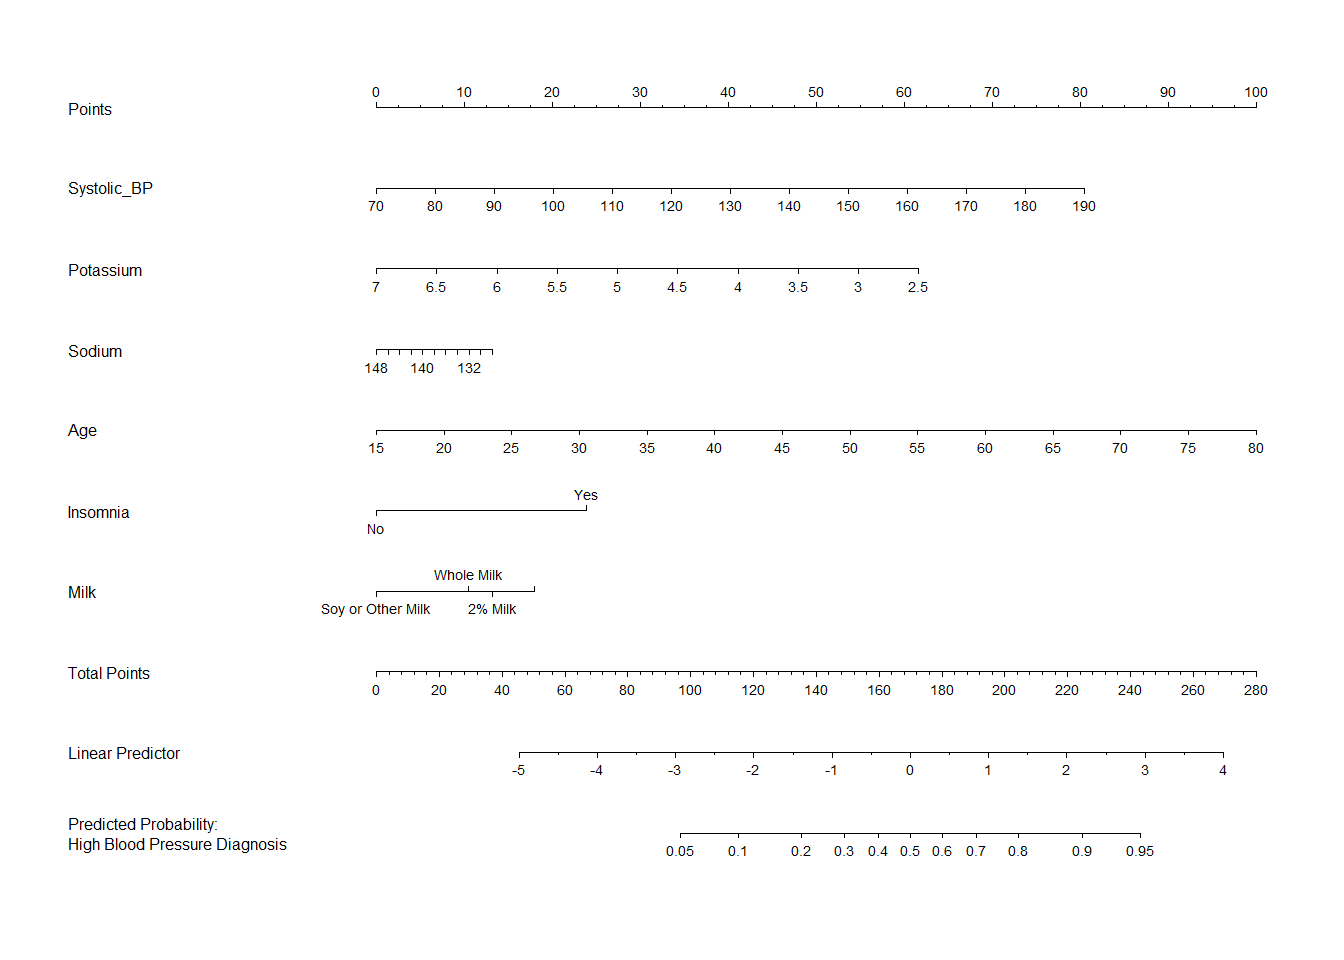
\includegraphics{project_A_presentation_slides_files/figure-beamer/unnamed-chunk-67-1.pdf}
\end{frame}

\hypertarget{logistic-regression}{%
\section{Logistic Regression}\label{logistic-regression}}

\begin{frame}[fragile]{Framingham Data (from Class 10)}
\protect\hypertarget{framingham-data-from-class-10}{}
\begin{Shaded}
\begin{Highlighting}[]
\NormalTok{fram\_raw }\OtherTok{\textless{}{-}} \FunctionTok{read\_csv}\NormalTok{(}\FunctionTok{here}\NormalTok{(}\StringTok{"data/framingham.csv"}\NormalTok{)) }\SpecialCharTok{\%\textgreater{}\%}
    \FunctionTok{type.convert}\NormalTok{(}\AttributeTok{as.is =} \ConstantTok{FALSE}\NormalTok{) }\SpecialCharTok{\%\textgreater{}\%}
    \FunctionTok{clean\_names}\NormalTok{() }
\end{Highlighting}
\end{Shaded}

The variables describe n = 4238 adults examined at baseline, then
followed for 10 years to see if they developed incident coronary heart
disease. The binary outcome (below) has no missing values.

\begin{Shaded}
\begin{Highlighting}[]
\NormalTok{fram\_raw }\SpecialCharTok{\%\textgreater{}\%} \FunctionTok{tabyl}\NormalTok{(ten\_year\_chd)}
\end{Highlighting}
\end{Shaded}

\begin{verbatim}
 ten_year_chd    n   percent
            0 3594 0.8480415
            1  644 0.1519585
\end{verbatim}
\end{frame}

\begin{frame}[fragile]{Data Cleanup}
\protect\hypertarget{data-cleanup}{}
\begin{Shaded}
\begin{Highlighting}[]
\NormalTok{fram\_new }\OtherTok{\textless{}{-}}\NormalTok{ fram\_raw }\SpecialCharTok{\%\textgreater{}\%}
    \FunctionTok{rename}\NormalTok{(}\AttributeTok{cigs =} \StringTok{"cigs\_per\_day"}\NormalTok{,}
           \AttributeTok{stroke =} \StringTok{"prevalent\_stroke"}\NormalTok{,}
           \AttributeTok{hrate =} \StringTok{"heart\_rate"}\NormalTok{,}
           \AttributeTok{sbp =} \StringTok{"sys\_bp"}\NormalTok{,}
           \AttributeTok{chd10\_n =} \StringTok{"ten\_year\_chd"}\NormalTok{) }\SpecialCharTok{\%\textgreater{}\%}
    \FunctionTok{mutate}\NormalTok{(}\AttributeTok{educ =} \FunctionTok{fct\_recode}\NormalTok{(}\FunctionTok{factor}\NormalTok{(education), }
                     \StringTok{"Some HS"} \OtherTok{=} \StringTok{"1"}\NormalTok{,}
                     \StringTok{"HS grad"} \OtherTok{=} \StringTok{"2"}\NormalTok{,}
                     \StringTok{"Some Coll"} \OtherTok{=} \StringTok{"3"}\NormalTok{,}
                     \StringTok{"Coll grad"} \OtherTok{=} \StringTok{"4"}\NormalTok{)) }\SpecialCharTok{\%\textgreater{}\%}
    \FunctionTok{mutate}\NormalTok{(}\AttributeTok{chd10\_f =} \FunctionTok{fct\_recode}\NormalTok{(}\FunctionTok{factor}\NormalTok{(chd10\_n),}
                     \StringTok{"chd"} \OtherTok{=} \StringTok{"1"}\NormalTok{, }\StringTok{"chd\_no"} \OtherTok{=} \StringTok{"0"}\NormalTok{)) }\SpecialCharTok{\%\textgreater{}\%}
    \FunctionTok{select}\NormalTok{(subj\_id, chd10\_n, chd10\_f, age, }
\NormalTok{           cigs, educ, hrate, sbp, stroke)}
\end{Highlighting}
\end{Shaded}
\end{frame}

\begin{frame}[fragile]{Data Descriptions}
\protect\hypertarget{data-descriptions}{}
Today, we'll only use the \texttt{chd} variables, plus \texttt{age}.

\begin{longtable}[]{@{}rl@{}}
\toprule
Variable & Description \\
\midrule
\endhead
\texttt{subj\_id} & identifying code added by Dr.~Love \\
\texttt{chd10\_n} & (numeric) 1 = coronary heart disease in next 10
years \\
\texttt{chd10\_f} & (factor) ``chd'' or ``chd\_no'' in next ten years \\
\texttt{age} & in years (range is 32 to 70) \\
\texttt{cigs} & number of cigarettes smoked per day \\
\texttt{educ} & 4-level factor: educational attainment \\
\texttt{hrate} & heart rate in beats per minute \\
\texttt{sbp} & systolic blood pressure in mm Hg \\
\texttt{stroke} & 1 = history of stroke, else 0 \\
\bottomrule
\end{longtable}
\end{frame}

\begin{frame}[fragile]{Missing Data?}
\protect\hypertarget{missing-data}{}
\begin{Shaded}
\begin{Highlighting}[]
\FunctionTok{miss\_var\_summary}\NormalTok{(fram\_new)}
\end{Highlighting}
\end{Shaded}

\begin{verbatim}
# A tibble: 9 x 3
  variable n_miss pct_miss
  <chr>     <int>    <dbl>
1 educ        105   2.48  
2 cigs         29   0.684 
3 hrate         1   0.0236
4 subj_id       0   0     
5 chd10_n       0   0     
6 chd10_f       0   0     
7 age           0   0     
8 sbp           0   0     
9 stroke        0   0     
\end{verbatim}
\end{frame}

\begin{frame}[fragile]{Prepare our outcome.}
\protect\hypertarget{prepare-our-outcome.}{}
We have our binary outcome as both a factor variable and a numeric (0/1)
variable

\begin{Shaded}
\begin{Highlighting}[]
\NormalTok{fram\_new }\SpecialCharTok{\%$\%} \FunctionTok{str}\NormalTok{(chd10\_f)}
\end{Highlighting}
\end{Shaded}

\begin{verbatim}
 Factor w/ 2 levels "chd_no","chd": 1 1 1 2 1 1 2 1 1 1 ...
\end{verbatim}

\begin{Shaded}
\begin{Highlighting}[]
\NormalTok{fram\_new }\SpecialCharTok{\%$\%} \FunctionTok{str}\NormalTok{(chd10\_n)}
\end{Highlighting}
\end{Shaded}

\begin{verbatim}
 int [1:4238] 0 0 0 1 0 0 1 0 0 0 ...
\end{verbatim}

\begin{Shaded}
\begin{Highlighting}[]
\NormalTok{fram\_new }\SpecialCharTok{\%\textgreater{}\%} \FunctionTok{tabyl}\NormalTok{(chd10\_f, chd10\_n)}
\end{Highlighting}
\end{Shaded}

\begin{verbatim}
 chd10_f    0   1
  chd_no 3594   0
     chd    0 644
\end{verbatim}
\end{frame}

\begin{frame}{Working with Binary Outcome Models}
\protect\hypertarget{working-with-binary-outcome-models}{}
Does Pr(CHD in next ten years) look higher for \emph{older} or
\emph{younger} people?

\includegraphics{project_A_presentation_slides_files/figure-beamer/unnamed-chunk-74-1.pdf}

\begin{longtable}[]{@{}lrrrr@{}}
\toprule
chd10\_f & n & mean(age) & sd(age) & median(age) \\
\midrule
\endhead
chd\_no & 3594 & 48.77 & 8.41 & 48 \\
chd & 644 & 54.15 & 8.01 & 55 \\
\bottomrule
\end{longtable}
\end{frame}

\begin{frame}[fragile]{So what do we expect in this model?}
\protect\hypertarget{so-what-do-we-expect-in-this-model}{}
Pr(CHD in next ten years) looks higher for \emph{older} people?

If we predict log(odds(CHD in next ten years)), we want to ensure that
value will be \textbf{rising} with increased age.

So, for the \texttt{mage\_1} model below, what sign do we expect for the
slope of \texttt{age}?

\begin{Shaded}
\begin{Highlighting}[]
\NormalTok{mage\_1 }\OtherTok{\textless{}{-}} \FunctionTok{glm}\NormalTok{(chd10\_f }\SpecialCharTok{\textasciitilde{}}\NormalTok{ age, }\AttributeTok{family =}\NormalTok{ binomial, }
              \AttributeTok{data =}\NormalTok{ fram\_new)}
\end{Highlighting}
\end{Shaded}
\end{frame}

\begin{frame}[fragile]{Results for \texttt{mage\_1}}
\protect\hypertarget{results-for-mage_1}{}
\begin{Shaded}
\begin{Highlighting}[]
\FunctionTok{tidy}\NormalTok{(mage\_1) }\SpecialCharTok{\%\textgreater{}\%} \FunctionTok{kable}\NormalTok{(}\AttributeTok{digits =} \DecValTok{3}\NormalTok{)}
\end{Highlighting}
\end{Shaded}

\begin{longtable}[]{@{}lrrrr@{}}
\toprule
term & estimate & std.error & statistic & p.value \\
\midrule
\endhead
(Intercept) & -5.558 & 0.284 & -19.585 & 0 \\
age & 0.075 & 0.005 & 14.166 & 0 \\
\bottomrule
\end{longtable}

\begin{Shaded}
\begin{Highlighting}[]
\FunctionTok{tidy}\NormalTok{(mage\_1, }\AttributeTok{exponentiate =} \ConstantTok{TRUE}\NormalTok{) }\SpecialCharTok{\%\textgreater{}\%} \FunctionTok{kable}\NormalTok{(}\AttributeTok{digits =} \DecValTok{3}\NormalTok{)}
\end{Highlighting}
\end{Shaded}

\begin{longtable}[]{@{}lrrrr@{}}
\toprule
term & estimate & std.error & statistic & p.value \\
\midrule
\endhead
(Intercept) & 0.004 & 0.284 & -19.585 & 0 \\
age & 1.077 & 0.005 & 14.166 & 0 \\
\bottomrule
\end{longtable}
\end{frame}

\begin{frame}[fragile]{Six ways to specify the outcome for this model}
\protect\hypertarget{six-ways-to-specify-the-outcome-for-this-model}{}
\begin{Shaded}
\begin{Highlighting}[]
\NormalTok{x1 }\OtherTok{\textless{}{-}} \FunctionTok{glm}\NormalTok{(chd10\_f }\SpecialCharTok{\textasciitilde{}}\NormalTok{ age, }
          \AttributeTok{family =}\NormalTok{ binomial, }\AttributeTok{data =}\NormalTok{ fram\_new)}
\NormalTok{x2 }\OtherTok{\textless{}{-}} \FunctionTok{glm}\NormalTok{(chd10\_n }\SpecialCharTok{\textasciitilde{}}\NormalTok{ age, }
          \AttributeTok{family =}\NormalTok{ binomial, }\AttributeTok{data =}\NormalTok{ fram\_new)}
\NormalTok{x3 }\OtherTok{\textless{}{-}} \FunctionTok{glm}\NormalTok{((chd10\_n }\SpecialCharTok{==} \StringTok{"1"}\NormalTok{) }\SpecialCharTok{\textasciitilde{}}\NormalTok{ age, }
          \AttributeTok{family =}\NormalTok{ binomial, }\AttributeTok{data =}\NormalTok{ fram\_new)}
\NormalTok{x4 }\OtherTok{\textless{}{-}} \FunctionTok{glm}\NormalTok{((chd10\_n }\SpecialCharTok{==} \StringTok{"0"}\NormalTok{) }\SpecialCharTok{\textasciitilde{}}\NormalTok{ age, }
          \AttributeTok{family =}\NormalTok{ binomial, }\AttributeTok{data =}\NormalTok{ fram\_new)}
\NormalTok{x5 }\OtherTok{\textless{}{-}} \FunctionTok{glm}\NormalTok{((chd10\_f }\SpecialCharTok{==} \StringTok{"chd"}\NormalTok{) }\SpecialCharTok{\textasciitilde{}}\NormalTok{ age, }
          \AttributeTok{family =}\NormalTok{ binomial, }\AttributeTok{data =}\NormalTok{ fram\_new)}
\NormalTok{x6 }\OtherTok{\textless{}{-}} \FunctionTok{glm}\NormalTok{((chd10\_f }\SpecialCharTok{==} \StringTok{"chd\_no"}\NormalTok{) }\SpecialCharTok{\textasciitilde{}}\NormalTok{ age, }
          \AttributeTok{family =}\NormalTok{ binomial, }\AttributeTok{data =}\NormalTok{ fram\_new)}
\end{Highlighting}
\end{Shaded}

What will happen to the \texttt{age} coefficient in these models?
\end{frame}

\begin{frame}[fragile]{Age Models \texttt{x1} and \texttt{x2}}
\protect\hypertarget{age-models-x1-and-x2}{}
\begin{Shaded}
\begin{Highlighting}[]
\NormalTok{x1 }\OtherTok{\textless{}{-}} \FunctionTok{glm}\NormalTok{(chd10\_f }\SpecialCharTok{\textasciitilde{}}\NormalTok{ age, }
          \AttributeTok{family =}\NormalTok{ binomial, }\AttributeTok{data =}\NormalTok{ fram\_new)}
\FunctionTok{extract\_eq}\NormalTok{(x1, }\AttributeTok{use\_coefs =} \ConstantTok{TRUE}\NormalTok{)}
\end{Highlighting}
\end{Shaded}

\begin{equation}
\log\left[ \frac { \widehat{P( \operatorname{chd10\_f} = \operatorname{chd} )} }{ 1 - \widehat{P( \operatorname{chd10\_f} = \operatorname{chd} )} } \right] = -5.56 + 0.07(\operatorname{age})
\end{equation}

\begin{Shaded}
\begin{Highlighting}[]
\NormalTok{x2 }\OtherTok{\textless{}{-}} \FunctionTok{glm}\NormalTok{(chd10\_n }\SpecialCharTok{\textasciitilde{}}\NormalTok{ age, }
          \AttributeTok{family =}\NormalTok{ binomial, }\AttributeTok{data =}\NormalTok{ fram\_new)}
\FunctionTok{extract\_eq}\NormalTok{(x2, }\AttributeTok{use\_coefs =} \ConstantTok{TRUE}\NormalTok{)}
\end{Highlighting}
\end{Shaded}

\begin{equation}
\log\left[ \frac { \widehat{P( \operatorname{chd10\_n} = \operatorname{1} )} }{ 1 - \widehat{P( \operatorname{chd10\_n} = \operatorname{1} )} } \right] = -5.56 + 0.07(\operatorname{age})
\end{equation}
\end{frame}

\begin{frame}[fragile]{Age Models \texttt{x3} and \texttt{x4}}
\protect\hypertarget{age-models-x3-and-x4}{}
\begin{Shaded}
\begin{Highlighting}[]
\NormalTok{x3 }\OtherTok{\textless{}{-}} \FunctionTok{glm}\NormalTok{((chd10\_n }\SpecialCharTok{==} \StringTok{"1"}\NormalTok{) }\SpecialCharTok{\textasciitilde{}}\NormalTok{ age, }
          \AttributeTok{family =}\NormalTok{ binomial, }\AttributeTok{data =}\NormalTok{ fram\_new)}
\FunctionTok{extract\_eq}\NormalTok{(x3, }\AttributeTok{use\_coefs =} \ConstantTok{TRUE}\NormalTok{)}
\end{Highlighting}
\end{Shaded}

\begin{equation}
\log\left[ \frac { \widehat{P( \operatorname{chd10\_n} = \operatorname{1} )} }{ 1 - \widehat{P( \operatorname{chd10\_n} = \operatorname{1} )} } \right] = -5.56 + 0.07(\operatorname{age})
\end{equation}

\begin{Shaded}
\begin{Highlighting}[]
\NormalTok{x4 }\OtherTok{\textless{}{-}} \FunctionTok{glm}\NormalTok{((chd10\_n }\SpecialCharTok{==} \StringTok{"0"}\NormalTok{) }\SpecialCharTok{\textasciitilde{}}\NormalTok{ age, }
          \AttributeTok{family =}\NormalTok{ binomial, }\AttributeTok{data =}\NormalTok{ fram\_new)}
\FunctionTok{extract\_eq}\NormalTok{(x4, }\AttributeTok{use\_coefs =} \ConstantTok{TRUE}\NormalTok{)}
\end{Highlighting}
\end{Shaded}

\begin{equation}
\log\left[ \frac { \widehat{P( \operatorname{chd10\_n} = \operatorname{0} )} }{ 1 - \widehat{P( \operatorname{chd10\_n} = \operatorname{0} )} } \right] = 5.56 - 0.07(\operatorname{age})
\end{equation}
\end{frame}

\begin{frame}[fragile]{Age Models \texttt{x5} and \texttt{x6}}
\protect\hypertarget{age-models-x5-and-x6}{}
\begin{Shaded}
\begin{Highlighting}[]
\NormalTok{x5 }\OtherTok{\textless{}{-}} \FunctionTok{glm}\NormalTok{((chd10\_f }\SpecialCharTok{==} \StringTok{"chd"}\NormalTok{) }\SpecialCharTok{\textasciitilde{}}\NormalTok{ age, }
          \AttributeTok{family =}\NormalTok{ binomial, }\AttributeTok{data =}\NormalTok{ fram\_new)}
\FunctionTok{extract\_eq}\NormalTok{(x5, }\AttributeTok{use\_coefs =} \ConstantTok{TRUE}\NormalTok{)}
\end{Highlighting}
\end{Shaded}

\begin{equation}
\log\left[ \frac { \widehat{P( \operatorname{chd10\_f} = \operatorname{chd} )} }{ 1 - \widehat{P( \operatorname{chd10\_f} = \operatorname{chd} )} } \right] = -5.56 + 0.07(\operatorname{age})
\end{equation}

\begin{Shaded}
\begin{Highlighting}[]
\NormalTok{x6 }\OtherTok{\textless{}{-}} \FunctionTok{glm}\NormalTok{((chd10\_f }\SpecialCharTok{==} \StringTok{"chd\_no"}\NormalTok{) }\SpecialCharTok{\textasciitilde{}}\NormalTok{ age, }
          \AttributeTok{family =}\NormalTok{ binomial, }\AttributeTok{data =}\NormalTok{ fram\_new)}
\FunctionTok{extract\_eq}\NormalTok{(x6, }\AttributeTok{use\_coefs =} \ConstantTok{TRUE}\NormalTok{)}
\end{Highlighting}
\end{Shaded}

\begin{equation}
\log\left[ \frac { \widehat{P( \operatorname{chd10\_f} = \operatorname{chd\_no} )} }{ 1 - \widehat{P( \operatorname{chd10\_f} = \operatorname{chd\_no} )} } \right] = 5.56 - 0.07(\operatorname{age})
\end{equation}
\end{frame}

\begin{frame}[fragile]{Making Predictions with a \texttt{glm} model}
\protect\hypertarget{making-predictions-with-a-glm-model}{}
\begin{Shaded}
\begin{Highlighting}[]
\NormalTok{modelL1 }\OtherTok{\textless{}{-}} \FunctionTok{glm}\NormalTok{(chd10\_f }\SpecialCharTok{==} \StringTok{"chd"} \SpecialCharTok{\textasciitilde{}}\NormalTok{ age, }
               \AttributeTok{family =}\NormalTok{ binomial, }\AttributeTok{data =}\NormalTok{ fram\_new)}

\NormalTok{new\_folks }\OtherTok{\textless{}{-}} \FunctionTok{tibble}\NormalTok{(}\AttributeTok{name =} \FunctionTok{c}\NormalTok{(}\StringTok{"Frank"}\NormalTok{, }\StringTok{"Grace"}\NormalTok{),}
                    \AttributeTok{age =} \FunctionTok{c}\NormalTok{(}\DecValTok{42}\NormalTok{, }\DecValTok{56}\NormalTok{))}

\NormalTok{new\_folks }\SpecialCharTok{\%\textgreater{}\%} \FunctionTok{kable}\NormalTok{()}
\end{Highlighting}
\end{Shaded}

\begin{longtable}[]{@{}lr@{}}
\toprule
name & age \\
\midrule
\endhead
Frank & 42 \\
Grace & 56 \\
\bottomrule
\end{longtable}
\end{frame}

\begin{frame}[fragile]{Predictions from a \texttt{glm} model
(\texttt{modelL1})}
\protect\hypertarget{predictions-from-a-glm-model-modell1}{}
\begin{block}{predictions on the logit scale}
\protect\hypertarget{predictions-on-the-logit-scale}{}
\begin{Shaded}
\begin{Highlighting}[]
\FunctionTok{predict}\NormalTok{(modelL1, }\AttributeTok{newdata =} \FunctionTok{data.frame}\NormalTok{(new\_folks))}
\end{Highlighting}
\end{Shaded}

\begin{verbatim}
        1         2 
-2.424935 -1.380563 
\end{verbatim}
\end{block}

\begin{block}{or on the probability scale (reminder: \texttt{glm} fit)}
\protect\hypertarget{or-on-the-probability-scale-reminder-glm-fit}{}
\begin{Shaded}
\begin{Highlighting}[]
\FunctionTok{predict}\NormalTok{(modelL1, }\AttributeTok{newdata =} \FunctionTok{data.frame}\NormalTok{(new\_folks),}
        \AttributeTok{type =} \StringTok{"response"}\NormalTok{)}
\end{Highlighting}
\end{Shaded}

\begin{verbatim}
        1         2 
0.0812909 0.2009186 
\end{verbatim}
\end{block}
\end{frame}

\begin{frame}[fragile]{Building a different model with \texttt{lrm}}
\protect\hypertarget{building-a-different-model-with-lrm}{}
\begin{Shaded}
\begin{Highlighting}[]
\NormalTok{dd }\OtherTok{\textless{}{-}} \FunctionTok{datadist}\NormalTok{(fram\_new)}
\FunctionTok{options}\NormalTok{(}\AttributeTok{datadist =} \StringTok{"dd"}\NormalTok{)}

\NormalTok{modelL2 }\OtherTok{\textless{}{-}} \FunctionTok{lrm}\NormalTok{(chd10\_f }\SpecialCharTok{==} \StringTok{"chd"} \SpecialCharTok{\textasciitilde{}} \FunctionTok{rcs}\NormalTok{(age, }\DecValTok{4}\NormalTok{), }
               \AttributeTok{data =}\NormalTok{ fram\_new, }\AttributeTok{x =} \ConstantTok{TRUE}\NormalTok{, }\AttributeTok{y =} \ConstantTok{TRUE}\NormalTok{)}
\end{Highlighting}
\end{Shaded}
\end{frame}

\begin{frame}[fragile]{Plot Effect Sizes from \texttt{modelL2}}
\protect\hypertarget{plot-effect-sizes-from-modell2}{}
\begin{Shaded}
\begin{Highlighting}[]
\FunctionTok{plot}\NormalTok{(}\FunctionTok{summary}\NormalTok{(modelL2))}
\end{Highlighting}
\end{Shaded}

\includegraphics{project_A_presentation_slides_files/figure-beamer/unnamed-chunk-89-1.pdf}
\end{frame}

\begin{frame}[fragile]{Making Predictions with \texttt{lrm}
(\texttt{modelL2})}
\protect\hypertarget{making-predictions-with-lrm-modell2}{}
\begin{Shaded}
\begin{Highlighting}[]
\NormalTok{new\_folks }\SpecialCharTok{\%\textgreater{}\%} \FunctionTok{kable}\NormalTok{()}
\end{Highlighting}
\end{Shaded}

\begin{longtable}[]{@{}lr@{}}
\toprule
name & age \\
\midrule
\endhead
Frank & 42 \\
Grace & 56 \\
\bottomrule
\end{longtable}

\begin{itemize}
\tightlist
\item
  Predictions on the logit scale
\end{itemize}

\begin{Shaded}
\begin{Highlighting}[]
\FunctionTok{predict}\NormalTok{(modelL2, }\AttributeTok{newdata =} \FunctionTok{data.frame}\NormalTok{(new\_folks))}
\end{Highlighting}
\end{Shaded}

\begin{verbatim}
        1         2 
-2.465157 -1.344158 
\end{verbatim}
\end{frame}

\begin{frame}[fragile]{Useful Predictions with \texttt{lrm}
(\texttt{modelL2})}
\protect\hypertarget{useful-predictions-with-lrm-modell2}{}
\begin{Shaded}
\begin{Highlighting}[]
\NormalTok{new\_folks }\SpecialCharTok{\%\textgreater{}\%} \FunctionTok{kable}\NormalTok{()}
\end{Highlighting}
\end{Shaded}

\begin{longtable}[]{@{}lr@{}}
\toprule
name & age \\
\midrule
\endhead
Frank & 42 \\
Grace & 56 \\
\bottomrule
\end{longtable}

\begin{itemize}
\tightlist
\item
  Predicted probabilities after an \texttt{lrm} fit\ldots{}
\end{itemize}

\begin{Shaded}
\begin{Highlighting}[]
\FunctionTok{predict}\NormalTok{(modelL2, }\AttributeTok{newdata =} \FunctionTok{data.frame}\NormalTok{(new\_folks),}
        \AttributeTok{type =} \StringTok{"fitted"}\NormalTok{)}
\end{Highlighting}
\end{Shaded}

\begin{verbatim}
         1          2 
0.07833722 0.20682714 
\end{verbatim}
\end{frame}

\begin{frame}[fragile]{Using the Nomogram to predict for Age 50}
\protect\hypertarget{using-the-nomogram-to-predict-for-age-50}{}
\begin{Shaded}
\begin{Highlighting}[]
\FunctionTok{plot}\NormalTok{(}\FunctionTok{nomogram}\NormalTok{(modelL2, }\AttributeTok{fun =}\NormalTok{ plogis))}
\end{Highlighting}
\end{Shaded}

\includegraphics{project_A_presentation_slides_files/figure-beamer/unnamed-chunk-94-1.pdf}
\end{frame}

\begin{frame}[fragile]{Compare our results from the nomogram\ldots{}}
\protect\hypertarget{compare-our-results-from-the-nomogram}{}
\begin{itemize}
\tightlist
\item
  Predicted probabilities after an \texttt{lrm} fit\ldots{}
\end{itemize}

\begin{Shaded}
\begin{Highlighting}[]
\FunctionTok{predict}\NormalTok{(modelL2, }\AttributeTok{newdata =} \FunctionTok{data.frame}\NormalTok{(}\AttributeTok{age =} \DecValTok{50}\NormalTok{),}
        \AttributeTok{type =} \StringTok{"fitted"}\NormalTok{)}
\end{Highlighting}
\end{Shaded}

\begin{verbatim}
        1 
0.1542483 
\end{verbatim}
\end{frame}

\begin{frame}[fragile]{Validate C statistic, Nagelkerke \(R^2\), Brier
score}
\protect\hypertarget{validate-c-statistic-nagelkerke-r2-brier-score}{}
\begin{Shaded}
\begin{Highlighting}[]
\FunctionTok{set.seed}\NormalTok{(}\DecValTok{2022}\NormalTok{)}
\FunctionTok{validate}\NormalTok{(modelL2, }\AttributeTok{B =} \DecValTok{50}\NormalTok{)}
\end{Highlighting}
\end{Shaded}

\begin{center}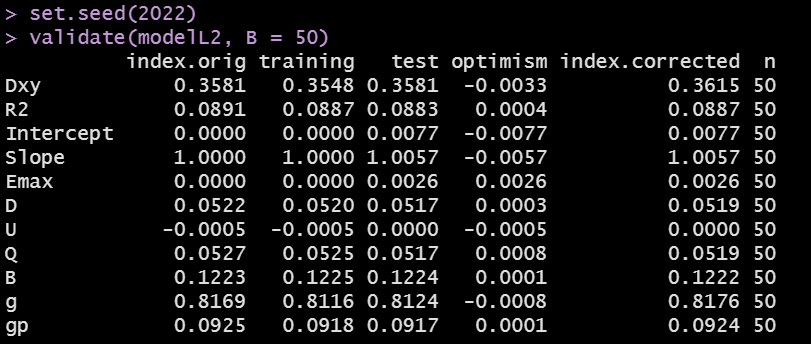
\includegraphics[width=0.9\linewidth]{figures/framval1} \end{center}
\end{frame}

\begin{frame}[fragile]{Next Time}
\protect\hypertarget{next-time}{}
\begin{itemize}
\tightlist
\item
  Logistic Regression using \texttt{tidymodels}
\item
  Quiz 1 will be made available today at 5 PM. Good luck!
\end{itemize}
\end{frame}

\end{document}
